\section{Hubs, costs, and markups: Berry, Carnall and Spiller (2006)}\label{sec:09-bcs}

\citet{BerryCarnallSpiller2006} bring the question of \cref{sec:09-borenstein} into the framework of
\cref{sec:09-pricing}. On ticket data of the same kind, they estimate a differentiated-products demand
system with two consumer types, a network model of marginal cost and a static Nash pricing equilibrium.
The model separates the two channels through which a hub can change the hub carrier's fares: higher markups
and lower costs. This section follows their analysis from the question to the conclusions, and
\cref{tab:09-bcs-map} at its end maps the study. As throughout the chapter, page, table, figure and footnote numbers refer to the 1996 working paper
\citep{BerryCarnallSpiller1996}.

\subsection{The question}\label{sec:09-bcs-question}

\Cref{sec:09-hubs} described the two views of hubs that coexisted by the mid-1980s. Critics held that hubs
raise entry barriers and fares for passengers who start their trips at a hub. Carriers and some economists
held that hubs reduce costs. The two effects are not mutually exclusive \citep{Berry1990}. A hub can raise
the markup over marginal cost for some travelers and lower marginal cost at the same time. On the demand
side, Berry, Carnall and
Spiller think of a hub as shifting out the demand for the hubbing carrier's flights out of its hub city.
Those flights may appeal especially to price-inelastic consumers, so the shift can also make demand less
elastic (p.~1). On the cost side, densely traveled spokes may have lower marginal costs. Economies of spoke
density then create economies of scope across itineraries that share a spoke (p.~2).

A fare regression cannot separate the two effects. Write the fare of product $j$ as $p_j=mc_j+m_j$, with
$m_j$ the markup. If hub presence raises $m_j$ and lowers $mc_j$, the change in the fare is
\begin{equation*}
\Delta p_j=\Delta m_j+\Delta mc_j,\qquad \Delta m_j>0,\quad \Delta mc_j<0 .
\end{equation*}
A regression of fares on hub presence estimates the sum. Without a model of markups or of costs it cannot
recover the two terms. As the authors note, \citet{Borenstein1989} has no model of costs or demand. In
their words, he ``attempts to control for market-level unobservables by, for example, introducing
city-pair level fixed effects'' (p.~5). His relative-price equation \eqref{eq:09-bor-rel} has the same
effect, since it differences out everything common to the carriers on an airport-pair route.
\citet{BruecknerSpiller1994} take the
opposite route. They estimate density economies from itineraries that pass through hubs without
originating there, to avoid hub markups (p.~4). That choice discards the markets where hub effects should
be largest. In the authors' words, reduced form regressions ``do not allow us to make statements about how
prices relate to costs, or what are the determinants of markups over cost'' (p.~6).

The strategy of the paper is to treat hub presence as one characteristic in a differentiated-products
model of demand. Combined with a cost model and an equilibrium assumption, the demand model yields a
markup for every product. Marginal cost is then ``observed'' as price minus the model's markup (p.~5), and
its relation to spoke density reveals economies of density. The model is the finite-mixture nested logit
of \cref{sec:09-pricing-types} with $R=2$ types, combined with the network costs of
\cref{sec:09-pricing-network}. The authors summarize their findings in five claims (abstract and
pp.~2--3), which we examine against their tables below.
\begin{enumerate}[label=(\roman*)]
  \item Travelers come in two distinct types. One has the attributes of a tourist: high price sensitivity
  and low willingness to pay for frequent-flyer features, frequency and nonstop service. The other has
  those of a business traveler.
  \item Hubs give the hub carrier two advantages: lower costs and higher markups on hub-originating
  passengers.
  \item The hub carrier's ability to raise prices is focused on business travelers. They shift toward the
  hub carrier even though they pay a premium of about 20\% over non-hub carriers.
  \item The hub carrier does not provide a ``monopoly umbrella'' to its rivals. Non-hub carriers lose
  business travelers and market share at the same time, which the authors call a ``competitive scissor.''
  \item There are economies of density on longer routes and none on routes shorter than about 500 miles,
  which the authors call the ``Southwest effect.''
\end{enumerate}

\subsection{Data}\label{sec:09-bcs-data}

The data come from the DOT ticket sample (DB1A) and the Service Segment Databank (DB27R) described in
\cref{sec:09-data}, for the fourth quarter of 1985 (p.~19). The quarter follows \citet{BruecknerDyerSpiller1992}
and \citet{BruecknerSpiller1994}. Those studies used only four-segment round trips that did not originate at
hub cities, to avoid demand-side hub effects. Berry, Carnall and Spiller model hub markups explicitly, so
they keep hub origins and itineraries with any number of segments up to two per direction. The ticket
conventions are those of \cref{sec:09-data}: round trips only, without itineraries chosen by a single
sampled passenger and without extreme fares. Southwest is absent, because it reported all its sales as one-way
tickets and so did not fit the product definition (p.~14, n.~11). The quarter precedes the merger wave of
1986--1987 and Borenstein's sample from 1987.

The unit of observation is a \emph{product} $j$, a unique combination of carrier, itinerary and fare in a
directional city-pair market $t$ (\cref{sec:09-data}). The sample has 122,871 products in 14,122 markets.
The products use 4,963 distinct carrier legs, flown by 32 carriers out of 262 origins, and represent
1,107,894 sampled passengers (p.~19). About 30\% of the markets have a single product and another 30\% have
no more than five. About 1\% have more than one hundred products, with a maximum of 874 in the New York to
Miami market. The quantity $q_{jt}$ is the number of sampled passengers (NPASS) and the price $p_{jt}$ is
the round-trip fare (FARE). Market size is built from $\mathit{MPOP}_t$, the geometric mean of the two
endpoint populations, $\sqrt{\text{origin population}\times\text{destination population}}$ (Appendix). A
\emph{leg} $\ell$ is a nonstop segment flown by one carrier. Its density $Q_\ell$ comes from DB27R and
adds the two directions, because the trips are round trips (Appendix, n.~4).

A structural model has more than one dependent variable. Each product contributes two endogenous outcomes,
its market share and its fare, and leg densities are endogenous as well. The inversion of demand turns the
share into the demand error $\xi_{jt}$. The pricing condition turns the fare into the cost error
$\omega_{jt}$. The regressors are the product and market characteristics in \cref{tab:09-bcs-vars} and the
leg cost terms. The instruments are discussed in \cref{sec:09-bcs-estimation}.

\begin{table}[htbp]
\centering
\begin{threeparttable}
\caption{Variables in the model of Berry, Carnall and Spiller}
\label{tab:09-bcs-vars}
\footnotesize
\begin{tabularx}{\textwidth}{@{}>{\raggedright\arraybackslash}p{2.2cm}>{\raggedright\arraybackslash}X
  >{\raggedright\arraybackslash}p{2.6cm}@{}}
\toprule
Variable & Definition (units) & Role \\
\midrule
\multicolumn{3}{@{}l}{\textit{Demand side (product $j$ of carrier $f$ in market $t$)}}\\
FARE & Round-trip fare (\$100) & Type-specific ($\alpha_r$) \\
DIRECT & 1 if the itinerary has one segment, 0 if it has two & Type-specific \\
HUBSIZE & If the origin is a hub of carrier $f$: the sum of the population potentials of all city pairs
  that $f$ connects through that hub. Zero otherwise & Type-specific \\
TEMPDIFF & Difference between the mean January temperatures of origin and destination (10\textdegree F) &
  Type-specific, market level \\
TRIPS-D & Minimum over the itinerary's legs of $f$'s departures on the leg (1,000 per quarter) &
  Type-specific \\
CONSTANT & 1 & Common \\
CONGEST-D & Number of endpoints (0, 1 or 2) that are slot controlled & Common, market level \\
MDIST, MDIST$^2$ & Great-circle distance between the endpoints (1,000 miles), and its square & Common, market
  level \\
\addlinespace
\multicolumn{3}{@{}l}{\textit{Cost side (summed over the legs $\ell\in\mathcal{L}(j)$ of the itinerary)}}\\
NSEGS & Number of legs (1 or 2) & Leg constant \\
CONGEST-S & Takeoffs and landings at the four slot-controlled airports (0 to 4) & Leg cost shifter \\
CONGEST-C & Takeoffs and landings at the 24 airports under FAA flow control (0 to 4) & Leg cost shifter \\
DIST, DENS & Leg distance $d_\ell$ (1,000 miles) and leg density $Q_\ell$ (100,000 passengers per quarter,
  both directions), with powers and interactions & Cubic polynomial \\
TRIPS-C & Leg departures $F_\ell$ (1,000 per quarter) & Column IV only \\
\bottomrule
\end{tabularx}
\begin{tablenotes}\footnotesize
\item Notes: The population potential of a city pair is the geometric mean of the two populations. The
slot-controlled airports are Chicago O'Hare, New York Kennedy and La Guardia, and Washington National
(p.~20, n.~13). The flow-control list includes Orange County and Long Beach (p.~21, n.~14). The text calls
the slot-control count CONGEST-C and the flow-control count DOT-CONGEST, while Tables 3 and 5 label the
cost-side congestion variables CONGEST-S and CONGEST-C. We match the labels by their sample means in
Table~3 (0.315 and 1.766), which equal the appendix means of the slot-control count (0.3149) and of the
flow-control count (1.7656). Source: \citet{BerryCarnallSpiller1996}, pp.~20--21 and Appendix.
\end{tablenotes}
\end{threeparttable}
\end{table}

\Cref{tab:09-bcs-desc} reproduces the descriptive statistics. The mean round-trip fare is \$276 with a
standard deviation of \$149. The number of sampled passengers per product has mean 9.0, standard deviation
31.3 and maximum 2,798, so most products are bought by very few sampled passengers. This fact matters for
the sampling error discussed in \cref{sec:09-bcs-estimation}. Slightly fewer than half of the products
(46.6\%) have a single segment. HUBSIZE is zero for most products, with mean 0.017 and standard deviation
0.045. Second-leg distances and densities are set to zero for one-segment products (p.~21), which explains
their low means. In the appendix statistics the means of DIRECT and NSEGS are 0.4666602 and 1.5333398,
which sum to exactly two, and their standard deviations are identical. In this sample DIRECT therefore
equals $2-\mathit{NSEGS}$, so ``direct'' means a single segment.

\begin{table}[htbp]
\centering
\begin{threeparttable}
\caption{Descriptive statistics, 122,871 origin-destination-fare-carrier products}
\label{tab:09-bcs-desc}
\small
\begin{tabular}{@{}lrrrr@{}}
\toprule
Variable & Mean & Std.\ dev. & Min & Max \\
\midrule
FARE (\$100) & 2.764 & 1.488 & 0.110 & 18.33 \\
NPASS (passengers) & 9.017 & 31.299 & 1.000 & 2798.0 \\
DIRECT (fraction) & 0.466 & 0.498 & 0.000 & 1.000 \\
HUBSIZE & 0.017 & 0.045 & 0.000 & 0.210 \\
TEMPDIFF (10\textdegree F) & 0.286 & 2.077 & $-6.520$ & 6.520 \\
TRIPS-D (minimum, 1,000 per quarter) & 0.293 & 0.179 & 0.001 & 1.595 \\
CONGEST-D (number of airports) & 0.202 & 0.413 & 0.000 & 2.000 \\
MDIST (1,000 miles) & 1.009 & 0.608 & 0.030 & 2.776 \\
\addlinespace
DIST, first outbound leg (1,000 miles) & 0.710 & 0.503 & 0.021 & 2.704 \\
DIST, second outbound leg (1,000 miles) & 0.351 & 0.479 & 0.000 & 2.611 \\
DENS, first outbound leg (100,000 per quarter) & 0.593 & 0.475 & 0.00003 & 4.553 \\
DENS, second outbound leg (100,000 per quarter) & 0.361 & 0.493 & 0.000 & 4.553 \\
TRIPS-C, first leg (1,000 departures per quarter) & 0.349 & 0.214 & 0.001 & 1.595 \\
TRIPS-C, second leg (1,000 departures per quarter) & 0.212 & 0.249 & 0.000 & 1.594 \\
\bottomrule
\end{tabular}
\begin{tablenotes}\footnotesize
\item Notes: Statistics across products. Second-leg values are zero for one-segment products.
Source: \citet{BerryCarnallSpiller1996}, Table~1.
\end{tablenotes}
\end{threeparttable}
\end{table}

The raw correlations among the endogenous variables point the wrong way for a naive test of density
economies (Table~2). Price is positively correlated with the densities of the first and second outbound legs
(0.084 and 0.122). Price and the number of passengers are negatively correlated ($-0.063$). The number of
passengers is correlated with the first-leg density at 0.068 and with the second-leg density at $-0.120$,
and the two densities are correlated at 0.164. The authors read the positive price-density correlations as
evidence that one must control for markups and distance before economies of density can appear (p.~21). One
reason is that dense legs connect large cities and hubs, where demand and markups may be high. In a
subsample of small four-segment markets, the sampling frame of Brueckner and Spiller, the raw correlation
between price and density is negative (p.~21, n.~15).

\subsection{Demand}\label{sec:09-bcs-demand}

\casehead{Market size}
The model needs an outside good, and hence a number of potential trips in each market. Berry, Carnall and
Spiller assume that this number is proportional to the geometric mean of the endpoint populations,
$M_t=\kappa\,\mathit{MPOP}_t$, with $\kappa$ a parameter to be estimated (p.~9). Each potential trip is
treated as a separate consumer, with no correlation of tastes across trips by the same person. The
observed shares are therefore functions of $\kappa$:
\begin{equation}\label{eq:09-bcs-sobs}
s^{obs}_{jt}(\kappa)=\frac{q_{jt}}{\kappa\,\mathit{MPOP}_t},\qquad
s^{obs}_{0t}(\kappa)=1-\sum_{j\in\mathcal{J}_t}s^{obs}_{jt}(\kappa).
\end{equation}
Because $q_{jt}$ counts passengers in a 10\% sample, $\kappa$ also absorbs the sampling rate.

\casehead{Unobserved product characteristics}
The term $\xi_{jt}$ captures ticket restrictions, such as advance-purchase and Saturday-stay requirements,
together with unmeasured quality such as food and service (p.~9). Firms and consumers observe it. Tickets
with different restrictions have systematically different prices, so $\xi_{jt}$ is correlated with price
by construction and price is endogenous. The authors assume instead that $\xi_{jt}$ is mean independent of
the other observed characteristics, such as distance and DIRECT. They defend this assumption with an
extreme case. Suppose every carrier offers the same menu of restrictions on every itinerary, for example
an unrestricted fare, an advance-purchase fare with a Saturday stay, and an advance-purchase fare without
one. Then the restrictiveness of a ticket is unrelated to $x_{jt}$. The authors concede that ``it is not
hard to think of stories which would violate'' the assumption (p.~9). A hub carrier that sells relatively
more unrestricted fares out of its hub would be one such story, since $\xi_{jt}$ would then rise with
HUBSIZE.

\casehead{Utility}
A potential traveler $i$ in market $t$ is of type $r\in\{1,2\}$, with $\Pr(r=1)=\psi$ and $\Pr(r=2)=1-\psi$.
In the notation of \cref{ass:09-fm}, a type-$r$ traveler has utility
\begin{equation}\label{eq:09-bcs-utility}
u_{ijt}=\delta^r_{jt}+\zeta_{igt}+(1-\sigma)\epsilon_{ijt}\quad(j\in\mathcal{J}_t),\qquad
u_{i0t}=\epsilon_{i0t},
\end{equation}
with type-specific mean utility
\begin{equation}\label{eq:09-bcs-delta-r}
\begin{aligned}
\delta^r_{jt}={}&\beta_0+\beta^{M}\mathit{MDIST}_t+\beta^{MM}\mathit{MDIST}_t^2+\beta^{C}\mathit{CONGEST\text{-}D}_t\\
&+\beta^{D}_r\mathit{DIRECT}_j+\beta^{h}_r\mathit{HUBSIZE}_{jt}+\beta^{T}_r\mathit{TEMPDIFF}_t
+\beta^{F}_r\mathit{TRIPS\text{-}D}_j-\alpha_rp_{jt}+\xi_{jt}.
\end{aligned}
\end{equation}
All inside goods form one nest and the outside good forms the other. Berry, Carnall and Spiller write the
idiosyncratic term as $\nu_i(\lambda)+\lambda\epsilon_{ij}$ (p.~11). In our notation $\lambda=1-\sigma$,
their $\nu_i(\lambda)$ is $\zeta_{igt}$, their type-1 probability $\gamma$ is $\psi$, and their market-size
factor $\mu$ is $\kappa$. As $\sigma\to0$ the choices within a market become uncorrelated and the model
reduces to a mixture of two logits. As $\sigma\to1$ the correlation of choices within the market goes to
one (p.~12).

\casehead{Shares}
Specializing \eqref{eq:09-fm-shares} to two types, the shares of a type-1 traveler are (p.~12)
\begin{equation}\label{eq:09-bcs-shares}
s^1_{j|g,t}=\frac{e^{\frac{\delta^1_{jt}}{1-\sigma}}}{D_{1t}},\qquad
D_{1t}=\sum_{k\in\mathcal{J}_t}e^{\frac{\delta^1_{kt}}{1-\sigma}},\qquad
\bar s_{1t}=\frac{D_{1t}^{1-\sigma}}{1+D_{1t}^{1-\sigma}},\qquad
s^1_{jt}=s^1_{j|g,t}\,\bar s_{1t},
\end{equation}
and the type-2 shares have the same form with $\delta^2_{jt}$. The predicted share of product $j$ is the
type-weighted average
\begin{equation}\label{eq:09-bcs-sj}
s_{jt}=\psi\,s^1_{jt}(p_t,x_t,\xi_t)+(1-\psi)\,s^2_{jt}(p_t,x_t,\xi_t).
\end{equation}

\casehead{Why two types}
\Cref{sec:09-pricing-types} gave the reasons why business travelers are less sensitive to price than
leisure travelers and why tastes are correlated across characteristics (p.~10, n.~9). A two-point
distribution is the simplest
bimodal distribution with correlated tastes (p.~10). The fat upper tail of fares per mile discussed in
\cref{sec:09-data} supports it. A mixture of two normal distributions fits that distribution far better than a
single normal. The authors compare the two components of that mixture with the estimated
model (p.~11, n.~10). The components are $N(0.2375, 0.0781)$ and $N(0.5946, 0.2752)$, so the second is
also far more dispersed. The model's mean fare per mile for type 1, 0.237, equals the mean of the first
component (0.2375). For type 2 the model gives 0.414, against 0.589 from the mixture.\footnote{The fitted
formula in footnote~10 gives the second component a mean of 0.5946, while the comparison in the same
footnote quotes 0.589. Likewise, the weight on the first component is 0.5987 in the formula and 0.598 in
the comparison. We report all four numbers as printed.} Type 1 accounts for 73\% of tickets in the model,
against a weight of 0.598 in the mixture. Five coefficients vary by type: those on FARE, DIRECT, HUBSIZE,
TEMPDIFF and TRIPS-D. By \cref{rem:09-discrete-rc}, two types need 11 parameters for these five
coefficients, against 10 for independent normal random coefficients, and they deliver closed-form shares.
The authors mention extensions they do not pursue (p.~11). Tastes could be drawn from two normal
distributions instead of two points, there could be more than two types, and nests could group airports
within a city or carriers within a market.

\casehead{The role of each characteristic}
The constant, MDIST, MDIST$^2$, CONGEST-D and TEMPDIFF are the same for every product in a market. They
shift the demand for air travel relative to the outside good (p.~20). They also cancel from each type's
within-nest shares $s^r_{j|g,t}$ in \eqref{eq:09-bcs-shares}. At given prices they therefore leave the
choice among flights of a traveler of either type unchanged. The paper concludes that TEMPDIFF ``has no
power to explain the choice between products'' (p.~20). This holds within a type. Aggregate shares can
still move, because these variables change the mix of types among the travelers who fly. By
\eqref{eq:09-bcs-sj}, the share of product $j$ among the inside goods is
\begin{equation*}
\frac{s_{jt}}{\sum_{k\in\mathcal{J}_t}s_{kt}}=\sum_{r=1}^{2}w_{rt}\,s^r_{j|g,t},\qquad
w_{1t}=\frac{\psi\,\bar s_{1t}}{\psi\,\bar s_{1t}+(1-\psi)\,\bar s_{2t}},\qquad w_{2t}=1-w_{1t},
\end{equation*}
where $w_{rt}$ is the share of type $r$ among the travelers who fly. A change in a market-level variable
leaves each $s^r_{j|g,t}$ fixed and moves the weights. If it raises every type-$r$ mean utility by $c_r$,
then $\frac{\partial\ln\bar s_{rt}}{\partial c_r}=1-\bar s_{rt}$. The weights therefore change when the
coefficient differs across types, as for TEMPDIFF. They also change under a common coefficient whenever
the two types' inside shares differ. The aggregate choice among flights then shifts toward the flights
that the type gaining weight prefers. DIRECT, HUBSIZE and TRIPS-D vary across carriers and itineraries within a market,
so they also govern substitution among flights within each type. HUBSIZE weights each city pair the carrier connects through its hub by
the pair's population potential. The authors prefer it to a hub dummy or to the number of points served,
neither of which accounts for the relative importance of the city pairs (p.~20). TEMPDIFF measures appeal to
tourists. Because its coefficient varies by type, it shifts the type mix and can help separate the types
(p.~20).

The model lets hub presence affect markups through the composition of buyers. By \eqref{eq:09-composition},
product $j$'s buyers are of type 2 with probability $\Pr(2\mid j)=\frac{(1-\psi)s^2_{jt}}{s_{jt}}$. By
\cref{prop:09-composition-markup} and \cref{rem:09-fm-extensions}, a single-product markup is close to
$\frac{1-\sigma}{\bar\alpha_j}$ when within-nest shares are small, where
$\bar\alpha_j=\Pr(1\mid j)\alpha_1+\Pr(2\mid j)\alpha_2$. If $\beta^h_2>\beta^h_1$ and $\alpha_2<\alpha_1$,
a larger HUBSIZE tilts the buyers of the hub carrier's products toward type 2, lowers $\bar\alpha_j$ and
raises the markup. Because $\Pr(2\mid j)$ is a logistic function of $\ln s^2_{jt}-\ln s^1_{jt}$, its shift
is proportional to $\Pr(2\mid j)\big(1-\Pr(2\mid j)\big)$ and is largest near an even mix. The markup
$\frac{1-\sigma}{\bar\alpha_j}$ is convex in $\Pr(2\mid j)$, however. With the column III price coefficients,
the markup response is largest for products whose buyers are already about 90\% type 2.

\subsection{Costs and pricing}\label{sec:09-bcs-supply}

\casehead{Leg costs and product marginal cost}
The cost side follows \citet{BruecknerSpiller1994}, as in \cref{sec:09-pricing-network}. Leg $\ell$ of carrier
$f$ has total cost $C_\ell(Q_\ell,w_\ell)$ and marginal cost $c_\ell(Q_\ell,w_\ell)$, where $w_\ell$
includes the leg's distance and the characteristics of its endpoint airports (p.~13). The carrier's cost is
\eqref{eq:09-firm-cost}, and the marginal cost of product $j$ is \eqref{eq:09-itin-mc}, the sum of its legs'
marginal costs plus a product-specific term $\omega_{jt}$. The authors give the product-specific cost the
form $\omega_{jt}q_{jt}$ only so that marginal cost has an additive error (p.~13). Fixed costs may also fall
with hubbing, but the model uses only marginal costs and cannot capture that effect.

\casehead{Prior beliefs about distance, density and frequency}
The authors expect a complicated relation among distance, density and flight frequency (pp.~13--14). On short
routes air travel competes with cars and, in a few places, trains. Carriers may then spend density savings
on more frequent flights, which let travelers choose departure times precisely. The East and West Coast
shuttles and Southwest are examples. On short routes large aircraft may also not pay, because takeoffs and
landings are a large share of cost. That cost does not vary with distance and is not offset by savings in
the air. The data have no model of frequency but do report quarterly trips on each leg. Frequency enters
some specifications as an exogenous cost shifter. These considerations call for a flexible functional form.

\casehead{The leg marginal cost function}
Segment marginal cost is a cubic polynomial in leg distance $d_\ell$ (1,000 miles) and leg density $Q_\ell$
(100,000 passengers per quarter), with congestion shifters. Write $\chi_{mn}$ for the coefficient on
$d_\ell^mQ_\ell^n$, and $n^S_\ell$ and $n^C_\ell$ for the leg's takeoffs and landings at slot-controlled and
at flow-control airports. In columns I to III of Table~5, leg marginal cost in \$100 is
\begin{equation}\label{eq:09-bcs-mc}
\begin{aligned}
c_\ell={}&\chi_{00}+\chi_{10}d_\ell+\chi_{20}d_\ell^2+\chi_{30}d_\ell^3
+\chi_{01}Q_\ell+\chi_{02}Q_\ell^2+\chi_{03}Q_\ell^3\\
&+\chi_{11}d_\ell Q_\ell+\chi_{21}d_\ell^2Q_\ell+\chi_{12}d_\ell Q_\ell^2
+\chi_S n^S_\ell+\chi_C n^C_\ell .
\end{aligned}
\end{equation}
Column IV adds nine terms in leg departures $F_\ell$ (1,000 per quarter):
\begin{equation}\label{eq:09-bcs-mc-trips}
\sum_{k=1}^{9}\chi^F_k\,h_k(F_\ell,d_\ell,Q_\ell),\qquad
(h_1,\dots,h_9)=(F,\,F^2,\,F^3,\,Fd,\,Fd^2,\,F^2d,\,FQ,\,F^2Q,\,FQ^2),
\end{equation}
with the leg subscripts dropped inside the list. Summing \eqref{eq:09-bcs-mc} over the legs of product $j$,
\begin{equation}\label{eq:09-bcs-mc-product}
mc_{jt}=\chi_{00}\,\mathit{NSEGS}_j+\chi_{10}\sum_{\ell\in\mathcal{L}(j)}d_\ell
+\dots+\chi_{12}\sum_{\ell\in\mathcal{L}(j)}d_\ell Q_\ell^2
+\chi_S\,\mathit{CONGEST\text{-}S}_j+\chi_C\,\mathit{CONGEST\text{-}C}_j+\omega_{jt}.
\end{equation}
The leg constant summed over legs becomes the coefficient on the number of segments. The mean of
$\omega_{jt}$, written $\bar\omega$, enters as a separate constant in product marginal cost (p.~21). Table~5
does not report it. Because NSEGS takes the values 1 and 2, $\bar\omega$ and $\chi_{00}$ are separately
identified.

Economies of density on leg $\ell$ mean that the leg's marginal cost falls as its density rises. From
\eqref{eq:09-bcs-mc},
\begin{equation}\label{eq:09-bcs-dcdq}
\frac{\partial c_\ell}{\partial Q_\ell}=\chi_{01}+2\chi_{02}Q_\ell+3\chi_{03}Q_\ell^2
+\chi_{11}d_\ell+\chi_{21}d_\ell^2+2\chi_{12}d_\ell Q_\ell ,
\end{equation}
and the leg has economies of density at $(d_\ell,Q_\ell)$ when this derivative is negative. In
\cref{ex:09-hubcost} the leg cost $aQ^\gamma$ has economies of density everywhere when $\gamma<1$. The
polynomial lets the sign vary with distance and density.

\casehead{What the cost model leaves out}
Prices, shares and densities are endogenous. Flight frequency is treated as exogenous. The data aggregate
traffic to the carrier, route and fare over a quarter, so they cannot show which flights are full or how
uncertainty about demand resolves before departure. The model therefore has no capacity constraints and no
demand uncertainty. The authors warn that ``some of what we label as a markup in fact represents a shadow
price of capacity'' (p.~14). Marginal cost may also vary with factors such as time-of-day capacity, which
the data do not record (p.~5).

\casehead{Pricing}
Following \citet{Berry1990}, prices form a static Nash equilibrium in which each carrier sets the prices of
all its products in all markets (pp.~6 and 14). The authors recognize that this is a simplification. Yield
management allocates seats across fare classes dynamically, and tacit collusion would add another layer,
but both are left for future work (p.~15). In the notation of \cref{sec:09-pricing-network}, carrier $f$'s
profit is (p.~15)
\begin{equation}\label{eq:09-bcs-profit}
\pi_f=\sum_t\ \sum_{j\in\mathcal{J}_f(t)}p_{jt}\,q_{jt}(p)-\sum_{\ell\in\mathcal{L}_f}C_\ell(Q_\ell,w_\ell)
-\sum_t\ \sum_{j\in\mathcal{J}_f(t)}\omega_{jt}\,q_{jt}(p)-FC_f .
\end{equation}
Differentiating with respect to $p_{jt}$ and exchanging the sums over legs and products, as in the
derivation of \eqref{eq:09-network-foc}, gives
\begin{equation}\label{eq:09-bcs-foc}
q_{jt}+\sum_{k\in\mathcal{J}_f(t)}\frac{\partial q_{kt}}{\partial p_{jt}}
\Big[p_{kt}-\omega_{kt}-\sum_{\ell\in\mathcal{L}(k)}c_\ell(Q_\ell,w_\ell)\Big]
=q_{jt}+\sum_{k\in\mathcal{J}_f(t)}\frac{\partial q_{kt}}{\partial p_{jt}}\,(p_{kt}-mc_{kt})=0 .
\end{equation}
Dividing by $M_t=\kappa\,\mathit{MPOP}_t$ turns quantities into shares. Stacking the conditions of market $t$
gives \eqref{eq:09-fm-markup}:
\begin{equation}\label{eq:09-bcs-markup}
p_t-mc_t=-\big[(\Omega_t\odot\Delta_t)^\top\big]^{-1}s_t,\qquad
\Delta_t=-\psi\,\alpha_1\frac{\partial s^1_t}{\partial\delta^1_t}-(1-\psi)\,\alpha_2\frac{\partial s^2_t}{\partial\delta^2_t},
\end{equation}
where the $(j,k)$ element of $\frac{\partial s^r_t}{\partial\delta^r_t}$ is given by
\eqref{eq:09-fm-derivs}.\footnote{The paper writes $p=\Delta^{-1}s+mc$ with $\Delta$ the matrix of
derivatives $\frac{\partial s_k}{\partial p_j}$ for products of the same firm (p.~15). That equation holds
when $\Delta$ contains the negatives of these derivatives. The paper's second expression,
$\Delta=\gamma\alpha_1\Delta_1+(1-\gamma)\alpha_2\Delta_2$ with $\Delta_r$ the derivatives with respect to
mean utility (p.~16), has the right sign. It equals $-(\Omega_t\odot\Delta_t)^\top$ in our notation. See
the footnote to \eqref{eq:09-fm-markup}.} Here $\Delta_t$ has $(j,k)$ element
$\frac{\partial s_{jt}}{\partial p_{kt}}$, as in \cref{ch:diffprod}.

Three features of \eqref{eq:09-bcs-markup} drive the empirical work. First, the markup depends only on the
demand parameters and on prices and shares (p.~16). It involves no cost parameter. Second, markups are not
profits. Airlines may be unprofitable even with large markups, because fixed costs may be large and marginal
cost may fall over a wide range of output (p.~16, \cref{rem:09-markups-profits}). Third, the network enters
the pricing condition only through the level of each $mc_{kt}$, evaluated at equilibrium densities.

\subsection{Estimation and identification}\label{sec:09-bcs-estimation}

\casehead{The estimator}
The parameters split into demand and cost parameters:
\begin{equation*}
\theta_d=(\sigma,\kappa,\psi,\alpha_1,\alpha_2,\beta_1,\beta_2),\qquad
\theta_c=(\bar\omega,\chi),\qquad \theta=(\theta_d,\theta_c).
\end{equation*}
Here $\beta_r$ collects type $r$'s taste coefficients, including the common
ones. The estimator follows \citet{Berry1994} and \citet{BerryLevinsohnPakes1995} (pp.~16--17). For a trial
value of $\theta$ it computes the two structural errors in five steps.
\begin{enumerate}[label=\arabic*.]
  \item Compute observed shares $s^{obs}_t(\kappa)$ from \eqref{eq:09-bcs-sobs}.
  \item Solve $s_t(\xi_t;\theta_d)=s^{obs}_t(\kappa)$ for $\xi_t(\theta_d)$ in each market, with the
  contraction \eqref{eq:09-fm-contraction}. \citet{Berry1994} guarantees a unique solution. The shares
  \eqref{eq:09-bcs-shares} and \eqref{eq:09-bcs-sj} are analytic, so no simulation is needed. With
  122,871 products the authors call this ``fortunate'' (p.~17).
  \item Evaluate $\Delta_t$ at $(p_t,\xi_t(\theta_d))$ and compute the markups
  $b_t(\theta_d)=-\big[(\Omega_t\odot\Delta_t)^\top\big]^{-1}s_t$ from \eqref{eq:09-bcs-markup}.
  \item Compute the cost error from \eqref{eq:09-bcs-mc-product}, with the observed densities as data:
  \begin{equation}\label{eq:09-bcs-omega}
  \tilde\omega_{jt}(\theta)=p_{jt}-b_{jt}(\theta_d)-\bar\omega-\sum_{\ell\in\mathcal{L}(j)}c_\ell(d_\ell,Q_\ell,n^S_\ell,n^C_\ell;\chi).
  \end{equation}
  \item Form the moments below and evaluate the objective.
\end{enumerate}
The identifying assumption is that both errors are mean independent of a vector of instruments $z_{jt}$:
\begin{equation}\label{eq:09-bcs-moments}
\E\left[\xi_{jt}(\theta_{d0})\given z_{jt}\right]=0,\qquad \E\left[\tilde\omega_{jt}(\theta_0)\given z_{jt}\right]=0 .
\end{equation}
With $N=122{,}871$ products and instrument matrices $Z^d_{jt}$ and $Z^c_{jt}$ built from $z_{jt}$, the
sample moments and the GMM estimator are
\begin{equation}\label{eq:09-bcs-gmm}
g_N(\theta)=\frac{1}{N}\sum_t\sum_{j\in\mathcal{J}_t}
\begin{pmatrix}Z^{d\top}_{jt}\,\xi_{jt}(\theta_d)\\ Z^{c\top}_{jt}\,\tilde\omega_{jt}(\theta)\end{pmatrix},
\qquad
\hat\theta=\argmin_\theta\ g_N(\theta)^\top W g_N(\theta),
\end{equation}
as in \cref{ch:blp}. Given $\theta_d$, the cost error is linear in $(\bar\omega,\chi)$. These parameters can
therefore be concentrated out by linear instrumental variables, like the linear parameters in
\cref{ch:blp}. The paper does not say how the search was organized.

\casehead{Instruments}
Price, shares and densities are endogenous. All other product and market characteristics are treated as
exogenous shifters of cost or demand, including the network structure of each carrier (pp.~17--18). The
instruments for leg densities include population and network characteristics at the endpoint cities. The
instruments for prices and markups add characteristics of the other products in the market (p.~18). The
authors chose the instrument vector by experimenting with simple versions of the model on a 10\% sample of
the data and then held it fixed for the full estimation (p.~18). The full list is not reported.

Each group of instruments rests on an economic argument. A product's own characteristics shift its demand
and, through the share, its markup. Rival products' characteristics shift the markup through the intensity
of competition, as in \citet{BerryLevinsohnPakes1995}. Population and network characteristics at the
endpoints shift a leg's density through traffic to and from other markets. Conditional on the included
characteristics, they are excluded from the product's own demand and cost errors. That exclusion requires
the network to be exogenous. If carriers built hubs where unobserved demand is high, network instruments
would be correlated with $\xi$. The paper does not model entry or network choice and refers to
\citet{Berry1990} and \citet{ReissSpiller1989} for that problem (p.~16, n.~12).

\casehead{Standard errors}
The errors are assumed independent across markets (p.~17). Within a market, demand and cost errors have a
factor structure, with market-specific components that are correlated across the demand and cost
equations. One parametrization consistent with this description is
\begin{equation}\label{eq:09-bcs-factor}
\xi_{jt}=a_t+e_{jt},\qquad \tilde\omega_{jt}=b_t+u_{jt},\qquad \Cov(a_t,b_t)\ne0,
\end{equation}
with $e_{jt}$ and $u_{jt}$ idiosyncratic. The structure enters the variance of the moments,
$V=\Var\big(\sum_{j\in\mathcal{J}_t}g_{jt}\big)$ summed over independent markets, where $g_{jt}$ is the
summand of \eqref{eq:09-bcs-gmm}. The asymptotic variance of $\hat\theta$ is then the usual sandwich
$(G^\top WG)^{-1}G^\top WVWG(G^\top WG)^{-1}$, with $G$ the derivative of the moments
(\cref{sec:A-gmm}). Treating each market as a cluster would be the nonparametric alternative.

\casehead{Sampling error in shares}
The inversion assumes that the econometrician observes expected shares \citep{Berry1994}. In
\citet{BerryLevinsohnPakes1995} shares were fractions of roughly 100 million households, so sampling error
was negligible. Here more than one million sampled passengers are spread over more than 120,000 products,
so the average product has fewer than 10 sampled passengers (p.~17). A rough calculation shows the
magnitude. If a product's sampled count $\hat n_j$ has mean $n_j$ and approximately Poisson variation, the
delta method gives $\Var(\ln\hat n_j)\approx\frac{1}{n_j}$. The standard deviation of the log share is then
about 0.33 at $n_j=9$ and 0.71 at $n_j=2$. By the derivative in the proof of
\cref{lem:09-fm-contraction}, $\frac{\partial\ln s_j}{\partial\xi_j}$ lies between $1-\max_r\bar s_r$ and
$\frac{1}{1-\sigma}$. It is close to one for the only product in a market, the case of about 30\% of markets
(p.~19). It is close to $\frac{1}{1-\sigma}$ when within-nest shares are small. An error in
$\ln s^{obs}_j$ therefore moves $\xi_j$ by between $1-\sigma$ and about one times the error. To first
order, random sampling noise has mean zero and is independent of the instruments. Three problems remain.
Standard errors that ignore the noise are too small. Because the logarithm is concave, $\ln\hat n_j$ has a
second-order bias of about $-\frac{1}{2n_j}$, which varies with expected sales and hence with the
instruments. The authors also drop itineraries chosen by a single sampled passenger (p.~19). This screen
applies to itineraries. It does not remove carrier-itinerary-fare products bought by one sampled passenger,
and Table~1 reports a minimum NPASS of 1.000 and a mean of 9.017. Their log shares carry the
largest sampling error, with a standard deviation near one by the Poisson approximation above. The itinerary
screen still selects the sample on sales, and sales vary with the instruments. The authors
leave the correction for future research (p.~17). \Cref{ch:blp} discusses the general problem.

\casehead{Identification of the types}
Some readers of early versions asked how market-level data can identify two unobserved types (p.~18). The
authors give two arguments, and the structure of the model supplies more.

The first argument concerns the price coefficients. \Cref{ex:09-twotypes} works it out with numbers. In a
model with one type and i.i.d.\ additive errors, two products with equal shares in one market must also have
equal shares when a third, similar product is added. With two types and flights that are close substitutes
within each type ($\sigma>0$), the cheap products compete for the same price-sensitive travelers. Adding a
cheap product then lowers the share of the cheap incumbent more than that of the expensive one. The farther apart the two price coefficients, the stronger this effect. Fares and
characteristics vary widely within and across markets (Table~1), so departures from the one-type model are
easy to detect (p.~18). The same mechanism makes the markup response depend on how similar the entrant
is. In a one-type model an entrant lowers markups only through the incumbent's own shares. Its effect then
depends on its mean utility. It does not depend on how close its price is to the incumbent's. In \cref{ex:09-twotypes},
$L$'s markup falls by 22\% under two types and by 9\% under one type.\footnote{The authors write that without
random coefficients ``markups and prices will not respond to the number of similar products in the market''
(p.~18). In a one-type model markups do fall with entry, through the incumbent's shares. The size of the
fall does not depend on the entrant's similarity.}

The second argument assigns the hub taste to the right type (pp.~18--19). HUBSIZE shifts the mean utility of
all products of carrier $f$ out of the origin. Summing the derivatives in \eqref{eq:09-fm-derivs} over
$k\in\mathcal{J}_f(t)$, for $j\in\mathcal{J}_f(t)$,
\begin{equation}\label{eq:09-bcs-hubid}
\frac{\partial\ln s_{jt}}{\partial\mathit{HUBSIZE}_{ft}}
=\sum_{r=1}^2\Pr(r\mid j)\,\beta^h_r\Big[\frac{1}{1-\sigma}-\frac{\sigma}{1-\sigma}S^r_{f|g,t}-S^r_{ft}\Big],
\end{equation}
where $S^r_{f|g,t}=\sum_{k\in\mathcal{J}_f(t)}s^r_{k|g,t}$ and $S^r_{ft}=\sum_{k\in\mathcal{J}_f(t)}s^r_{kt}$
are carrier $f$'s within-nest and total shares among type-$r$ travelers. For a given type the bracket is the
same for all of the carrier's products. Differences between the hub responses of a carrier's cheap and
expensive products therefore come only through the buyer weights $\Pr(r\mid j)$. The price coefficients pin
down these weights. If the price-sensitive type likes hubs more, the shares of cheap products respond more
to hub size, and conversely. Comparing the relative shares of cheap and expensive products of the same
carrier at hub and non-hub origins thus identifies $\beta^h_1$ and $\beta^h_2$ separately.

Three further sources of identification come from the structure. TEMPDIFF moves the inside share of each type
at a rate that depends on $\beta^T_r$ and so changes the type mix of a market's travelers. The demand
coefficient on DIRECT and the cost coefficient on NSEGS are separately identified even though
$\mathit{DIRECT}=2-\mathit{NSEGS}$. The first is pinned down by shares through $\xi$ and the second by prices
net of markups through $\omega$. Finally, the market-size factor $\kappa$ is identified mainly by functional
form, through how inside shares vary across markets of different size. Its large standard errors in
Table~5 reflect this.

\subsection{Results}\label{sec:09-bcs-results}

\subsubsection{A descriptive price regression}

Before estimating the model, Berry, Carnall and Spiller regress the fare on cost variables, and then on cost
and demand variables, by ordinary least squares (\cref{tab:09-bcs-ols}). The distance coefficient is 1.004,
about \$100 per 1,000 miles. Density has the expected sign but a small magnitude. An increase of 100,000
passengers per quarter in spoke density lowers the fare by about \$9 (p.~21). Adding demand variables makes
the density coefficient slightly more negative, from $-0.088$ to $-0.094$.\footnote{The text says instead that
the magnitude of the density coefficient ``decreases further'' when demand variables are added (p.~22). We
follow Table~3.} The $R^2$ is 0.173 without and 0.177 with the
demand variables, so observed costs and characteristics explain little of the variation in fares. The
HUBSIZE coefficient is 2.097 (0.094), which the authors describe as consistent with the ``Borenstein''
effect of hubs on markups (p.~22). By our arithmetic, a one standard deviation increase in HUBSIZE (0.045)
raises the fare by $2.097\times0.045=0.094$, or \$9.\footnote{The text also says that the coefficient on
DIRECT is ``fairly large, about \$75'' (p.~22), but Table~3 has no DIRECT row. Since DIRECT equals
$2-\mathit{NSEGS}$ in this sample, a regression that included NSEGS, DIRECT and a constant would be
perfectly collinear. We do not report the \$75 figure as an estimate.}

The authors stress that these regressions are ``for descriptive purposes only, as the estimated coefficients
bear little necessary relationship to the parameters of the model'' (p.~21). The reasons follow from
\cref{sec:09-bcs-supply}. The fare equals marginal cost plus a markup that depends on demand. Density is
endogenous. HUBSIZE can lower costs and raise markups at once. The OLS coefficient on HUBSIZE is the net
of the two, exactly the sum $\Delta m_j+\Delta mc_j$ of \cref{sec:09-bcs-question}.

\begin{table}[htbp]
\centering
\begin{threeparttable}
\caption{Ordinary least squares regressions of fare on cost and demand variables}
\label{tab:09-bcs-ols}
\small
\begin{tabular}{@{}lccc@{}}
\toprule
 & Cost only & Cost and demand & Mean \\
\midrule
CONSTANT & 1.704 (0.013) & 1.545 (0.022) & 1.000 \\
NSEGS & $-0.113$ (0.013) & $-0.011$ (0.017) & 1.533 \\
CONGEST-S & 0.084 (0.007) & 0.082 (0.008) & 0.315 \\
CONGEST-C & 0.012 (0.005) & 0.012 (0.005) & 1.766 \\
DIST & 1.004 (0.008) & 1.004 (0.008) & 1.062 \\
DENS & $-0.088$ (0.012) & $-0.094$ (0.012) & 0.954 \\
TRIPS-C & 0.362 (0.029) & 0.310 (0.037) & 0.561 \\
CONGEST-D & & 0.009 (0.013) & 0.202 \\
HUBSIZE & & 2.097 (0.094) & 0.017 \\
TEMPDIFF & & $-0.011$ (0.002) & 0.286 \\
TRIPS-D & & 0.019 (0.040) & 0.294 \\
\addlinespace
$R^2$ & 0.173 & 0.177 & \\
\bottomrule
\end{tabular}
\begin{tablenotes}\footnotesize
\item Notes: Dependent variable FARE in \$100. Standard errors in parentheses. Cost variables are sums over
the legs of the itinerary. The number of observations is not printed in the table. The sample is the
122,871 products of \cref{tab:09-bcs-desc}. Source: \citet{BerryCarnallSpiller1996}, Table~3.
\end{tablenotes}
\end{threeparttable}
\end{table}

\subsubsection{Demand estimates}

\Cref{tab:09-bcs-demand} reproduces the demand panel of Table~5 with the implied composition of travelers
from Table~4. Column I has a single type. Column II lets only the price coefficient differ across types.
Column III lets the coefficients on FARE, DIRECT, HUBSIZE, TEMPDIFF and TRIPS-D differ. Column IV keeps the
demand specification of column III and adds leg departures to marginal cost. The coefficient reported for
FARE multiplies minus the fare in \$100, so a positive value means that travelers dislike higher fares.

\begin{table}[htbp]
\centering
\begin{threeparttable}
\caption{Demand estimates and implied composition of travelers}
\label{tab:09-bcs-demand}
\footnotesize
\setlength{\tabcolsep}{4pt}
\begin{tabular}{@{}lcccc@{}}
\toprule
 & I & II & III & IV \\
 & One type & Types differ in price & Types differ & Column III with \\
 & & coefficient only & in five coefficients & trips in cost \\
\midrule
LAMBDA ($\lambda$) & 0.605 (0.020) & 0.638 (0.020) & 0.599 (0.027) & 0.617 (0.026) \\
$\sigma=1-\lambda$ & 0.395 (0.020) & 0.362 (0.020) & 0.401 (0.027) & 0.383 (0.026) \\
MU ($\kappa$) & 4.766 (0.464) & 8.652 (2.079) & 8.651 (2.471) & 9.532 (1.625) \\
PROB TYPE 1 ($\psi$) & 1.000 (fixed) & 0.924 (0.018) & 0.975 (0.013) & 0.952 (0.019) \\
\addlinespace
FARE 1 ($\alpha_1$) & 0.455 (0.039) & 0.696 (0.054) & 0.829 (0.075) & 0.986 (0.084) \\
FARE 2 ($\alpha_2$) & & 0.068 (0.014) & 0.077 (0.017) & 0.111 (0.024) \\
DIRECT 1 & 0.656 (0.023) & 0.542 (0.022) & 0.414 (0.060) & 0.293 (0.063) \\
DIRECT 2 & & & 1.014 (0.070) & 0.876 (0.070) \\
HUBSIZE 1 & 0.437 (0.026) & 0.213 (0.013) & 0.285 (0.047) & 0.615 (0.075) \\
HUBSIZE 2 & & & 0.761 (0.423) & 0.368 (0.127) \\
TEMPDIFF 1 & 0.050 (0.003) & 0.049 (0.003) & 0.052 (0.005) & 0.049 (0.007) \\
TEMPDIFF 2 & & & 0.049 (0.017) & 0.050 (0.016) \\
TRIPS-D 1 & 0.551 (0.058) & 0.393 (0.041) & 0.329 (0.055) & 0.388 (0.061) \\
TRIPS-D 2 & & & 0.954 (0.395) & 0.493 (0.231) \\
CONSTANT & $-10.305$ (0.034) & $-10.621$ (0.033) & $-10.207$ (0.034) & $-10.172$ (0.034) \\
CONGEST-D & $-0.158$ (0.030) & $-0.215$ (0.030) & $-0.186$ (0.031) & $-0.203$ (0.030) \\
MDIST & 0.528 (0.070) & 0.562 (0.069) & 0.772 (0.071) & 0.752 (0.070) \\
MDIST$^2$ & $-0.126$ (0.029) & $-0.176$ (0.028) & $-0.206$ (0.029) & $-0.209$ (0.029) \\
\midrule
\multicolumn{5}{@{}l}{\textit{Implied composition of travelers (Table 4)}}\\
Share of passengers, type 1 (\%) & 100 & 70.99 & 73.19 & 60.13 \\
Share of passengers, type 2 (\%) & & 29.01 & 26.81 & 39.87 \\
Share of population, type 1 (\%) & 100 & 92.35 & 97.48 & 95.21 \\
Share of population, type 2 (\%) & & 7.65 & 2.52 & 4.79 \\
Average fare, type 1 (\$) & & 205 & 204 & 191 \\
Average fare, type 2 (\$) & & 338 & 351 & 323 \\
Average $\xi$, type 1 & & 0.97 & 0.86 & 0.87 \\
Average $\xi$, type 2 & & 1.19 & 1.30 & 1.22 \\
Average trips, type 1 & & 0.39 & 0.37 & 0.39 \\
Average trips, type 2 & & 0.36 & 0.39 & 0.36 \\
\bottomrule
\end{tabular}
\begin{tablenotes}\footnotesize
\item Notes: GMM estimates, standard errors in parentheses. FARE coefficients multiply minus the fare in
\$100. In column II the type-2 coefficients other than FARE equal the type-1 coefficients. The row
$\sigma=1-\lambda$ converts the paper's nesting parameter to the book's convention and has the same
standard error. Table~4 prints 0.616 for the type-1 HUBSIZE coefficient in column IV. The averages in the
bottom panel weight products by predicted passengers of each type. Source:
\citet{BerryCarnallSpiller1996}, Table~5 (demand panel) and Table~4 (bottom panel).
\end{tablenotes}
\end{threeparttable}
\end{table}

\casehead{One type}
In column I the nesting parameter is $\sigma=0.395$ with a standard error of 0.020, so the pure logit
($\sigma=0$) is rejected with a $t$ statistic near 20 (p.~22). Choices among flights in a market are
correlated relative to the outside good. The other coefficients have the expected signs. Travelers prefer
direct flights, flights from uncongested airports and flights on the hubbing airline. The distance terms
have an inverse U shape. As distance rises, air travel becomes more attractive relative to driving, but the
total demand for travel may fall (p.~22). The inside utility peaks at
$\mathit{MDIST}=\frac{\beta^M}{2|\beta^{MM}|}$, which is $\frac{0.528}{2\times0.126}=2.10$ (2,095 miles) in
column I and $\frac{0.772}{2\times0.206}=1.87$ (1,874 miles) in column III.

\casehead{Two price coefficients}
In column II the type-1 price coefficient is $\frac{0.696}{0.068}=10.2$ times the type-2 coefficient, which
the authors describe as ``nearly ten times'' (p.~23). Price-sensitive travelers make up 92.4\% of potential
travelers but only 71\% of passengers. They are much less likely to buy a ticket at all.

\casehead{Five type-specific coefficients}
In column III the type-2 share of potential travelers falls from almost 8\% to 2.5\% (p.~23). Type 2 is a
small minority of the population but more than a quarter of passengers (26.8\%). Relative to type 1, type 2
cares more about direct flights (1.014 against 0.414), about hub size at the origin (0.761 against 0.285)
and about frequency (0.954 against 0.329). Its valuation of TEMPDIFF is a little lower (0.049 against 0.052)
and less precisely estimated. The authors conclude that ``the data and the model together can identify two
types of consumers that can sensibly be labeled `tourist' and `business'\,'' (p.~23). Two type-2
coefficients are imprecise. HUBSIZE 2 has a $t$ statistic of $\frac{0.761}{0.423}=1.8$ and TRIPS-D 2 one of
$\frac{0.954}{0.395}=2.4$.

\casehead{The column IV puzzle and willingness to pay}
In column IV the type-1 HUBSIZE coefficient (0.615) exceeds the type-2 coefficient (0.368). The authors call
this the only puzzling result and resolve it with marginal willingness to pay (p.~23). Utility is linear in
characteristics and price, so an indifference curve in the space of characteristic $k$ and fare satisfies
$\beta^k_r\,\dd x^k-\alpha_r\,\dd p=0$. Its slope is the marginal willingness to pay of type $r$, in dollars
when the fare is measured in \$100:
\begin{equation}\label{eq:09-bcs-wtp}
\mathit{WTP}^k_r=\frac{\dd p}{\dd x^k}\bigg|_{u_r\ \text{constant}}=\frac{\beta^k_r}{\alpha_r}\times\$100 .
\end{equation}
The nesting parameter scales both coefficients equally and does not enter. For HUBSIZE in column III,
\begin{equation*}
\mathit{WTP}^h_1=\frac{0.285}{0.829}\times\$100=\$34,\qquad
\mathit{WTP}^h_2=\frac{0.761}{0.077}\times\$100=\$988
\end{equation*}
per unit of HUBSIZE. In column IV the values are $\frac{0.615}{0.986}\times\$100=\$62$ and
$\frac{0.368}{0.111}\times\$100=\$332$. Type 2's willingness to pay for hub size is higher in both columns,
which removes the puzzle. HUBSIZE has no natural unit, so \cref{tab:09-bcs-wtp} also scales it by its
standard deviation, 0.045. A one standard deviation increase in HUBSIZE is worth \$1.55 to a tourist and
\$44.47 to a business traveler in column III.

\begin{table}[htbp]
\centering
\begin{threeparttable}
\caption{Marginal willingness to pay and price sensitivity implied by the demand estimates}
\label{tab:09-bcs-wtp}
\small
\begin{tabular}{@{}lcccc@{}}
\toprule
 & \multicolumn{2}{c}{Column III} & \multicolumn{2}{c}{Column IV} \\
\cmidrule(lr){2-3}\cmidrule(lr){4-5}
 & Type 1 & Type 2 & Type 1 & Type 2 \\
\midrule
DIRECT (\$ for a one-segment itinerary) & 50 & 1,317 & 30 & 789 \\
HUBSIZE (\$ per unit) & 34 & 988 & 62 & 332 \\
HUBSIZE (\$ per standard deviation, 0.045) & 1.55 & 44.47 & 2.81 & 14.92 \\
TRIPS-D (\$ per 1,000 departures per quarter) & 40 & 1,239 & 39 & 444 \\
TRIPS-D (\$ per standard deviation, 0.179) & 7.1 & 221.8 & 7.0 & 79.5 \\
TEMPDIFF (\$ per 10\textdegree F) & 6.3 & 63.6 & 5.0 & 45.0 \\
\addlinespace
$\frac{\alpha_r}{1-\sigma}$ (fall in a product's share per \$100, in logs) & 1.384 & 0.129 & 1.598 & 0.180 \\
\bottomrule
\end{tabular}
\begin{tablenotes}\footnotesize
\item Notes: Our computations from the Table~5 estimates. Willingness to pay is
$\frac{\beta^k_r}{\alpha_r}\times\$100$, from \eqref{eq:09-bcs-wtp}. Standard deviations of HUBSIZE and
TRIPS-D are from Table~1. The last row is the upper bound on the semi-elasticity of a type-$r$ traveler's
demand for a product, attained when the product's shares are small.
\end{tablenotes}
\end{threeparttable}
\end{table}

The dollar values for type 2 are large because its price coefficient is small. A business traveler is
almost indifferent to fares over the relevant range, so any characteristic it values has a large price
equivalent. The ratio of two estimates is also imprecise when the denominator is small. The type-2 price
coefficient in column III has a standard error of 0.017 on a value of 0.077. The ranking is the robust
finding: type 2 values hub size, directness and frequency far more than type 1 in every specification.

\casehead{Price sensitivity}
The last row of \cref{tab:09-bcs-wtp} translates the price coefficients into semi-elasticities. From
\eqref{eq:09-fm-derivs}, a type-$r$ traveler's demand for product $j$ falls by
$\alpha_r\big[\frac{1}{1-\sigma}-\frac{\sigma}{1-\sigma}s^r_{j|g}-s^r_j\big]$ log points per \$100, which is
at most $\frac{\alpha_r}{1-\sigma}$. In column III a \$10 fare increase therefore lowers a tourist's demand
for a product by at most 0.138 log points, about 13\%. It lowers a business traveler's demand by at most
0.013 log points, about 1.3\%. The elasticity of
aggregate demand for a product is the buyer-weighted average of the type elasticities
(\cref{sec:09-pricing-types}).

\casehead{Who travels}
Type 2 is 2.52\% of potential travelers and 26.81\% of passengers in column III. A type-2 potential traveler
is therefore $\frac{26.81}{2.52}\times\frac{97.48}{73.19}=14.2$ times as likely to fly as a type-1
potential traveler. The authors note that these proportions match a 1993
survey in which 8\% of air travelers accounted for 44\% of all trips (p.~24, n.~16). The mean fare paid by
type 1 is \$204, and type 2 pays almost \$150 more (\$351). Business travelers get something for the extra
dollars. Across all products $\xi$ has mean zero, but passengers favor high-quality tickets, so its mean
across tickets sold is about 0.98. It is about 30\% higher for type 2 and 12\% lower for type 1 (p.~24). The
Table~4 averages give $\frac{1.30}{0.98}=1.33$ and $\frac{0.86}{0.98}=0.88$. Business travelers buy tickets
with fewer restrictions and higher unmeasured quality.

\casehead{Stability across specifications}
The type structure is stable. Across columns II to IV, type 2 is 2.5\% to 7.7\% of potential travelers and
27\% to 40\% of passengers. The ratio of price coefficients is 10.2, 10.8 and 8.9. The type-2 willingness to
pay for hub size falls from \$988 in column III to \$332 in column IV, so its magnitude depends on the cost
specification. Tables 6 and 7 use column III only, and the paper reports no standard errors for them.

\subsubsection{Cost estimates}

\Cref{tab:09-bcs-cost} reproduces the cost panel of Table~5. The polynomial makes individual coefficients
hard to interpret (p.~23), so the authors summarize them through the derivative \eqref{eq:09-bcs-dcdq}
below. Several patterns are still visible. In columns I to III congestion raises leg marginal cost. In
column III each takeoff or landing at a slot-controlled airport adds \$6.0 and each at a flow-control airport
\$7.1. In column IV the slot-control coefficient turns negative ($-0.033$). The negative NSEGS coefficient
implies a negative intercept in leg marginal cost, which the authors read as a sign of problems with the
specification near zero distance and density (p.~23). The linear distance term is positive. The linear
density term is also positive, which by itself does not support economies of density. The interaction terms
nevertheless imply economies of density over a wide range (p.~24). Adding trips in column IV changes the
distance and density terms substantially. For example, the linear distance coefficient falls from 3.181 to
0.155, and the NSEGS coefficient becomes positive.

\begin{table}[htbp]
\centering
\begin{threeparttable}
\caption{Leg marginal cost estimates}
\label{tab:09-bcs-cost}
\footnotesize
\begin{tabular}{@{}llcccc@{}}
\toprule
Variable & Coefficient & I & II & III & IV \\
\midrule
NSEGS & $\chi_{00}$ & $-1.453$ (0.157) & $-0.922$ (0.088) & $-0.656$ (0.095) & 0.081 (0.234) \\
CONGEST-S & $\chi_S$ & 0.125 (0.030) & 0.046 (0.017) & 0.060 (0.019) & $-0.033$ (0.015) \\
CONGEST-C & $\chi_C$ & 0.041 (0.012) & 0.073 (0.007) & 0.071 (0.008) & 0.072 (0.010) \\
DIST & $\chi_{10}$ & 4.510 (0.395) & 2.965 (0.223) & 3.181 (0.241) & 0.155 (0.631) \\
DIST$^2$ & $\chi_{20}$ & $-2.117$ (0.241) & $-1.297$ (0.136) & $-1.420$ (0.147) & 1.117 (0.446) \\
DIST$^3$ & $\chi_{30}$ & 0.402 (0.044) & 0.168 (0.247) & 0.178 (0.027) & $-0.410$ (0.096) \\
DIST$\times$DENS & $\chi_{11}$ & $-5.229$ (0.794) & $-3.540$ (0.448) & $-3.891$ (0.486) & $-6.651$ (1.287) \\
DIST$^2\times$DENS & $\chi_{21}$ & 1.419 (0.254) & 1.045 (0.143) & 1.270 (0.155) & 2.986 (0.454) \\
DENSITY & $\chi_{01}$ & 2.060 (0.506) & 1.818 (0.282) & 1.584 (0.307) & 4.827 (1.259) \\
DENSITY$^2$ & $\chi_{02}$ & 0.376 (0.384) & $-0.252$ (0.213) & 0.164 (0.232) & 1.537 (0.522) \\
DENSITY$^3$ & $\chi_{03}$ & $-0.379$ (0.081) & $-0.102$ (0.046) & $-0.238$ (0.050) & $-1.012$ (0.341) \\
DENS$^2\times$DIST & $\chi_{12}$ & 1.140 (0.277) & 0.564 (0.156) & 0.524 (0.169) & 0.392 (0.361) \\
\addlinespace
TRIPS & $\chi^F_1$ & & & & $-4.544$ (2.536) \\
TRIPS$^2$ & $\chi^F_2$ & & & & 13.540 (4.826) \\
TRIPS$^3$ & $\chi^F_3$ & & & & $-13.612$ (2.524) \\
TRIPS$\times$DIST & $\chi^F_4$ & & & & 6.989 (3.868) \\
TRIPS$\times$DIST$^2$ & $\chi^F_5$ & & & & $-5.075$ (1.374) \\
TRIPS$^2\times$DIST & $\chi^F_6$ & & & & 4.913 (2.360) \\
TRIPS$\times$DENS & $\chi^F_7$ & & & & $-14.381$ (3.247) \\
TRIPS$^2\times$DENS & $\chi^F_8$ & & & & 9.237 (2.114) \\
TRIPS$\times$DENS$^2$ & $\chi^F_9$ & & & & 2.008 (1.605) \\
\bottomrule
\end{tabular}
\begin{tablenotes}\footnotesize
\item Notes: GMM estimates, standard errors in parentheses. Leg marginal cost in \$100, distance in 1,000
miles, density in 100,000 passengers per quarter, trips in 1,000 departures per quarter. The coefficient
names refer to \eqref{eq:09-bcs-mc} and \eqref{eq:09-bcs-mc-trips}. The standard error of DIST$^3$ in
column II is printed as 0.247. Source: \citet{BerryCarnallSpiller1996}, Table~5 (cost panel).
\end{tablenotes}
\end{threeparttable}
\end{table}

\subsubsection{Hubs, markups, and the sorting of travelers}

Table~6 turns the column III estimates into a comparison of hub and non-hub carriers. Its construction uses
the buyer composition \eqref{eq:09-composition}. For each product the model predicts the number of passengers
of each type, $\hat n_{jrt}=\hat\kappa\,\mathit{MPOP}_t\,\hat\psi_r\,\hat s^r_{jt}$, where $\hat\psi_1=\hat\psi$
and $\hat\psi_2=1-\hat\psi$. Because the model fits observed shares exactly, $\hat n_{jrt}=q_{jt}\Pr(r\mid j)$.

Markets are classified by the largest HUBSIZE among the carriers that serve them. HUBSIZE is zero for 93.5\%
of origin-carrier combinations. A \emph{non-hub market} has HUBSIZE equal to zero for every carrier. A
\emph{small-hub market} has a largest HUBSIZE strictly between 0 and 0.01. A \emph{large-hub market} has at
least one carrier with HUBSIZE of 0.01 or more, about the largest third of hubs. Within hub markets, a
\emph{hub carrier} has positive HUBSIZE at the origin and the others are non-hub carriers. The 778 markets
served only by hub carriers, with 5.2\% of passengers, are excluded.

For market category $m$, carrier group $h$ and type $r$, a characteristic $x$ such as the fare or marginal
cost is averaged in two steps. First, within each market $t$ it is averaged over the group's products with
weights equal to predicted type-$r$ passengers. Second, the market averages are averaged across the markets
in category $m$ with weights equal to total passengers $q_t$:
\begin{equation}\label{eq:09-bcs-avg}
\bar x_{t,h,r}=\frac{\sum_{j\in\mathcal{J}^h_t}\hat n_{jrt}\,x_{jt}}{\sum_{j\in\mathcal{J}^h_t}\hat n_{jrt}},
\qquad
\bar x_{m,h,r}=\frac{\sum_{t\in m}q_t\,\bar x_{t,h,r}}{\sum_{t\in m}q_t}.
\end{equation}
Averaging within markets first controls for differences across markets in distance, population and other
market characteristics. Levels remain hard to compare across market categories, so the authors focus on hub
and non-hub differences within a category (p.~25). In this subsection only, $F$ and $M$ denote the average
fare and marginal cost. They do not denote the number of carriers or market size here. Subscripts $H$ and $N$ mark hub and
non-hub carriers. The average markup is $\frac{F-M}{F}$,
and the three hub premia are
\begin{equation}\label{eq:09-bcs-premia}
\text{fare}=\frac{F_H-F_N}{F_N},\qquad
\text{marginal cost}=\frac{M_N-M_H}{M_N},\qquad
\text{markup}=\frac{(F_H-M_H)-(F_N-M_N)}{F_N-M_N}.
\end{equation}
The marginal-cost premium is positive when the hub carrier's cost is lower.\footnote{The table notes print
the markup premium without the inner brackets.}

\Cref{tab:09-bcs-hub} reproduces Table~6 with markets and carriers in rows. Panel B adds our recomputation of
the premia from the rounded averages. The printed premia use unrounded averages, so the two differ slightly.

\begin{table}[htbp]
\centering
\begin{threeparttable}
\caption{Fares, marginal costs and markups of hub and non-hub carriers (column III estimates)}
\label{tab:09-bcs-hub}
\footnotesize
\setlength{\tabcolsep}{2.8pt}
\begin{tabular}{@{}llcccccccccc@{}}
\toprule
\multicolumn{12}{@{}l}{\textit{Panel A. Averages by market type, customer type and carrier type}}\\
\midrule
Type & Carrier & Pct of & Pct of & Pct of & Fare & MC & Markup & Fare per & Avg & Avg & Avg \\
 & & market & car.\ tot. & type & (\$) & (\$) & (\%) & mile (\$) & $\xi$ & direct & trips \\
\midrule
\multicolumn{12}{@{}l}{Non-hub markets: 31\% of passengers, 82\% of markets, 800 miles}\\
1 & Non-hub & 75.8 & 100 & 100 & 224 & 93 & 58.6 & 0.387 & 0.601 & 0.522 & 336 \\
2 & Non-hub & 24.2 & 100 & 100 & 296 & 111 & 62.4 & 0.488 & 1.005 & 0.542 & 340 \\
\addlinespace
\multicolumn{12}{@{}l}{Small-hub markets: 32\% of passengers, 9\% of markets, 954 miles, population 3.8
million}\\
1 & Hub & \multirow{2}{*}{73.2} & 73.6 & 40.0 & 206 & 96 & 53.4 & 0.301 & 0.650 & 0.792 & 399 \\
1 & Non-hub & & 73.0 & 60.0 & 206 & 95 & 53.8 & 0.302 & 0.771 & 0.778 & 404 \\
2 & Hub & \multirow{2}{*}{26.8} & 26.4 & 39.3 & 306 & 111 & 63.7 & 0.398 & 0.942 & 0.809 & 410 \\
2 & Non-hub & & 27.0 & 60.7 & 295 & 106 & 63.9 & 0.398 & 1.074 & 0.819 & 430 \\
\addlinespace
\multicolumn{12}{@{}l}{Large-hub markets: 37\% of passengers, 9\% of markets, 842 miles, population 3.0
million}\\
1 & Hub & \multirow{2}{*}{70.4} & 67.0 & 62.3 & 215 & 91 & 57.8 & 0.336 & 0.875 & 0.922 & 469 \\
1 & Non-hub & & 76.8 & 37.7 & 205 & 109 & 46.7 & 0.313 & 0.566 & 0.622 & 362 \\
2 & Hub & \multirow{2}{*}{29.6} & 33.0 & 72.9 & 319 & 98 & 69.2 & 0.474 & 1.321 & 0.927 & 484 \\
2 & Non-hub & & 23.2 & 27.1 & 268 & 133 & 50.4 & 0.403 & 0.836 & 0.665 & 371 \\
\midrule
\multicolumn{12}{@{}l}{\textit{Panel B. Hub premia (\%), as printed and recomputed from the rounded averages of Panel A}}\\
\midrule
 & & \multicolumn{3}{c}{Printed} & \multicolumn{3}{c}{Recomputed} & & & & \\
\cmidrule(lr){3-5}\cmidrule(lr){6-8}
Market & Type & Fare & MC & Markup & Fare & MC & Markup & & & & \\
\midrule
Small hub & 1 & 0.1 & $-1.1$ & $-0.8$ & 0.0 & $-1.1$ & $-0.9$ & & & & \\
Small hub & 2 & 3.7 & $-4.5$ & 3.3 & 3.7 & $-4.7$ & 3.2 & & & & \\
Large hub & 1 & 5.0 & 16.8 & 29.9 & 4.9 & 16.5 & 29.2 & & & & \\
Large hub & 2 & 19.0 & 26.1 & 63.4 & 19.0 & 26.3 & 63.7 & & & & \\
\bottomrule
\end{tabular}
\begin{tablenotes}\footnotesize
\item Notes: Group headings give each market category's share of passengers and of markets, its average
market distance and, for hub markets, its average population. ``Pct of market'' is the share of the type
among the market category's passengers. ``Pct of
car.\ tot.'' is the share of the type among the carrier group's passengers. ``Pct of type'' is the share of
the type's passengers who fly the carrier group. Averages are computed as in \eqref{eq:09-bcs-avg}, markups
as $\frac{F-M}{F}$ and premia as in \eqref{eq:09-bcs-premia}. Average trips are departures per quarter. The
778 markets served only by hub carriers (5.2\% of passengers) are excluded. In non-hub markets the paper
prints 100 in the ``Pct of car.\ tot.'' column for both types. By the definition above, the type shares among
non-hub carriers there are 75.8\% and 24.2\%, as in the ``Pct of market'' column. The entries of 100 in the
``Pct of type'' column are correct, since every carrier in these markets is a non-hub carrier. Source:
\citet{BerryCarnallSpiller1996}, Table~6. Panel B recomputation: our computations.
\end{tablenotes}
\end{threeparttable}
\end{table}

\casehead{Market composition}
Non-hub markets are 82\% of markets but carry only 31\% of passengers (p.~25). The remaining passengers are
split almost evenly between small-hub and large-hub markets. Non-hub markets have the highest share of
tourists (75.8\%) and large-hub markets the highest share of business travelers (29.6\%).

\casehead{Small hubs}
In small-hub markets the two carrier groups look alike. Hub carriers carry 40.0\% of type-1 and 39.3\% of
type-2 passengers, so non-hub carriers carry 60\% of the market. The two groups have nearly identical
passenger mixes (26.4\% and 27.0\% type 2). Type 1 pays \$206 on both. Type 2 pays 3.7\% more on hub carriers,
whose marginal cost for type 2 is 4.5\% higher.\footnote{The text says that hub carriers in small-hub markets
have ``4\% lower marginal costs'' for type-2 travelers (p.~26). Table~6 shows a marginal cost of \$111 for
hub carriers against \$106 for non-hub carriers. Its marginal-cost premium of $-4.5\%$ means, by the table's
definition, a higher cost for hub carriers. We follow the table.} Non-hub carriers' products have
14\% to 18\% higher $\xi$ and more trips (p.~26).

\casehead{Large hubs}
In large-hub markets the hub premium appears. By our arithmetic on Table~6, hub carriers carry about 65\% of all
passengers: $0.704\times0.623+0.296\times0.729=0.654$. The product is exact if each ``Pct of type'' entry is an
aggregate share of the category's type-$r$ passengers. If the entries instead average market-level shares as in
\eqref{eq:09-bcs-avg}, the product omits cross-market covariances and is only an approximation. Hub carriers carry 72.9\% of business travelers and 62.3\% of
tourists, so their passengers are 33.0\% type 2 against 23.2\% for non-hub carriers (p.~25). Business
travelers pay \$319 on the hub carrier against \$268 on non-hub carriers, a premium of 19.0\%. The hub
carrier's marginal cost for these tickets is \$98 against \$133, an advantage of 26.1\%. Its markup per
ticket is therefore \$221 against \$135, which is 63.4\% higher (63.7\% from the rounded averages). Tourists
pay 5.0\% more on the hub carrier, which has a 16.8\% cost advantage and a 29.9\% higher markup. The
business-ticket Lerner index is 69.2\% for hub carriers and 50.4\% for non-hub carriers.

The fare premium can be decomposed into a markup gain and a cost advantage, both measured relative to the
non-hub fare. Subtracting and adding the two marginal costs,
\begin{equation}\label{eq:09-bcs-decomp}
\frac{F_H-F_N}{F_N}=\frac{(F_H-M_H)-(F_N-M_N)}{F_N}-\frac{M_N-M_H}{F_N}.
\end{equation}
For business travelers in large hubs this gives
\begin{equation*}
\frac{319-268}{268}=\frac{221-135}{268}-\frac{133-98}{268},\qquad\text{that is,}\qquad
19.0\%=32.1\%-13.1\% .
\end{equation*}
The hub carrier's markup gain exceeds its fare premium, because lower cost finances part of the markup. The
authors make the same point with different numbers, a 29\% markup premium net of a 10\% cost
advantage.\footnote{The text quotes the large-hub type-2 comparison as fares of ``\$305 vs.\ \$255'' and
average costs of ``\$94 vs.\ \$118,'' a cost advantage of 20\%. It gives markups of ``\$211 vs.\ \$137,'' or
53\% higher (p.~26). Table~6 gives fares of \$319 and \$268, marginal costs of \$98 and \$133 and premia of 19.0\%,
26.1\% and 63.4\%. Recomputing from the rounded Table~6 averages gives 19.0\%, 26.3\% and 63.7\%. The 29\%
and 10\% decomposition in the text follows from the text's numbers. We use the table throughout.}

Hub carriers in large hubs also sell different products. Their products are more often direct (0.922 and
0.927 against 0.622 and 0.665), have more departures (469 and 484 against 362 and 371) and have higher
$\xi$. Non-hub carriers' products have values of $\xi$ about 35\% smaller than those of hub carriers (p.~26).
Part of the hub premium is therefore a payment for directness, frequency and unmeasured quality, which
business travelers value most.

\begin{figure}[htbp]
\centering
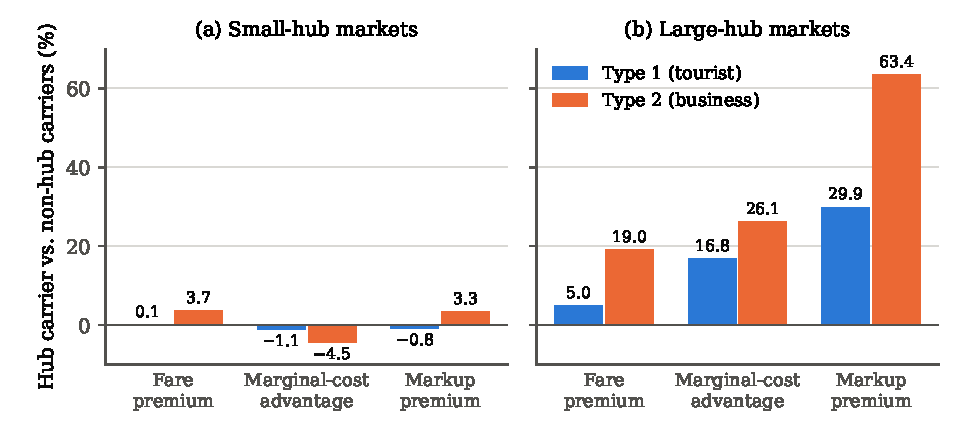
\includegraphics[width=\textwidth]{figures/ch09/bcs_hubpremia.pdf}
\caption{Hub premia by market and traveler type. The fare premium is the percentage by which the hub
carrier's average fare exceeds that of non-hub carriers. The marginal-cost advantage and the markup premium
are defined in \eqref{eq:09-bcs-premia}. Redrawn from the bottom panel of Table~6 of
\citet{BerryCarnallSpiller1996}, based on the column III estimates.}
\label{fig:09-bcs-premia}
\end{figure}

\Cref{fig:09-bcs-premia} plots the premia.\footnote{The text describes a Figure~4 that presents these
results (p.~26, n.~17), but the posted working paper does not contain it. Our figure plots the numbers of
Table~6 and does not reproduce Figure~4.} The pattern supports claims (ii) and (iii). In small hubs the
premia are close to zero for both types. In large hubs the hub carrier earns a substantial premium from
business travelers and a small one from tourists, while enjoying lower marginal cost for both. Business
travelers ``are not just willing to pay the 20\% premia that hub airlines charge,'' they also fly the hub
carrier more often than its rivals (p.~26).

\casehead{No umbrella: the competitive scissor}
The hub carrier's high fares do not protect its rivals. Non-hub carriers in large-hub markets charge less
than non-hub carriers in non-hub markets (\$205 against \$224 for tourists, \$268 against \$296 for business
travelers). They also lose the business travelers, so their passenger mix is more price sensitive (p.~27). Both
blades of the scissor lower their average yield and the profitability of serving the hub airport. This is
claim (iv), and it matches Borenstein's finding of little umbrella effect (\cref{sec:09-borenstein}). The
fare comparison runs across market categories, which the authors warn against elsewhere (p.~25). The
within-market evidence is cleaner: non-hub carriers' business fares are 16\% below the hub carrier's
($\frac{268}{319}=0.84$).

\casehead{A dynamic interpretation}
The authors suggest an explanation, untested in the paper, of two trends after deregulation (p.~27). Once a
carrier builds a major hub at an airport, its rivals see business customers move away and their yields fall.
Marginal carriers then find it profitable to cut service to that city, and airport concentration rises
without any entry barrier. \citet{BruecknerSpiller1994} document this rise. Hubs also give their carriers
price and cost advantages that ease entry out of the hub into new city pairs. That could explain the fall in
concentration at the level of city-pair markets. For empirical models of airline entry they refer to
\citet{ReissSpiller1989} and \citet{Berry1992}.\footnote{The text cites ``Berry (1991)'' here, while the
reference list contains \citet{Berry1992}, the published entry model.}

\subsubsection{Economies of density}

\Cref{tab:09-bcs-dmc} reproduces Table~7, the derivative of leg marginal cost with respect to density
\eqref{eq:09-bcs-dcdq} at column III estimates, for five distances and six densities. With the column III
coefficients the derivative is
\begin{equation}\label{eq:09-bcs-dcdq-III}
\frac{\partial c_\ell}{\partial Q_\ell}=1.584+2(0.164)Q_\ell+3(-0.238)Q_\ell^2-3.891d_\ell+1.270d_\ell^2
+2(0.524)d_\ell Q_\ell .
\end{equation}
Panel B of the table evaluates this formula. It reproduces 29 of the 30 printed cells to within 0.006, which
is rounding. The exception is the cell for 250 miles and density 1.50.\footnote{Table~7 prints $-0.27$ for
250 miles and 150,000 passengers per quarter. Formula \eqref{eq:09-bcs-dcdq-III} gives $-0.031$, which also
fits the neighboring cells (0.568 at density 1.00 and $-0.980$ at 2.00). We treat the printed value as a
typographical error.}

\begin{table}[htbp]
\centering
\begin{threeparttable}
\caption{Derivative of leg marginal cost with respect to density (column III)}
\label{tab:09-bcs-dmc}
\small
\begin{tabular}{@{}lrrrrrr@{}}
\toprule
 & \multicolumn{6}{c}{Leg density (100,000 passengers per quarter)} \\
\cmidrule(l){2-7}
Leg distance & 0.25 & 0.50 & 0.75 & 1.00 & 1.50 & 2.00 \\
\midrule
\multicolumn{7}{@{}l}{\textit{Panel A. As printed in Table 7}}\\
250 miles & 0.794 & 0.808 & 0.733 & 0.568 & $-0.27$ & $-0.980$ \\
500 miles & 0.125 & 0.204 & 0.194 & 0.096 & $-0.369$ & $-1.190$ \\
1,000 miles & $-0.737$ & $-0.527$ & $-0.406$ & $-0.373$ & $-0.576$ & $-1.135$ \\
1,500 miles & $-0.964$ & $-0.623$ & $-0.371$ & $-0.207$ & $-0.148$ & $-0.446$ \\
2,000 miles & $-0.556$ & $-0.084$ & 0.299 & 0.593 & 0.914 & 0.879 \\
\addlinespace
\multicolumn{7}{@{}l}{\textit{Panel B. Computed from the Table 5 column III coefficients}}\\
250 miles & 0.793 & 0.807 & 0.732 & 0.567 & $-0.031$ & $-0.985$ \\
500 miles & 0.124 & 0.203 & 0.193 & 0.094 & $-0.373$ & $-1.196$ \\
1,000 miles & $-0.738$ & $-0.527$ & $-0.407$ & $-0.375$ & $-0.579$ & $-1.141$ \\
1,500 miles & $-0.965$ & $-0.623$ & $-0.372$ & $-0.209$ & $-0.151$ & $-0.451$ \\
2,000 miles & $-0.557$ & $-0.084$ & 0.298 & 0.592 & 0.912 & 0.874 \\
\bottomrule
\end{tabular}
\begin{tablenotes}\footnotesize
\item Notes: \$100 per 100,000 passengers per quarter. A negative entry means economies of density. Panel B
evaluates \eqref{eq:09-bcs-dcdq-III} (our computations). Source:
\citet{BerryCarnallSpiller1996}, Table~7.
\end{tablenotes}
\end{threeparttable}
\end{table}

\begin{figure}[htbp]
\centering
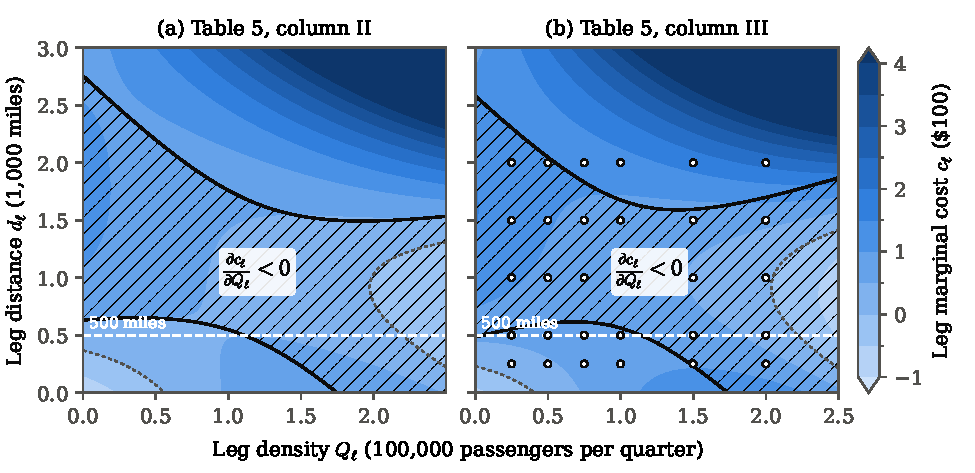
\includegraphics[width=\textwidth]{figures/ch09/bcs_mc_surface.pdf}
\caption{Leg marginal cost over leg density and distance. Shading gives the level of $c_\ell$ in \$100 from
\eqref{eq:09-bcs-mc}, with congestion terms and the product-level constant set to zero. The hatched region,
bounded by the solid curve, has $\frac{\partial c_\ell}{\partial Q_\ell}<0$ (economies of density). Dotted
curves mark $c_\ell=0$, where the polynomial turns negative. The dashed line marks 500 miles, and the dots in
panel (b) are the grid points of \cref{tab:09-bcs-dmc}. Leg densities above 250,000 passengers per
quarter, up to the observed maximum of 455,300, are not shown. Constructed from
\citet{BerryCarnallSpiller1996}, Table~5, columns II and III.}
\label{fig:09-bcs-mc}
\end{figure}

\Cref{fig:09-bcs-mc} redraws the cost surface for columns II and III. The working paper shows the same
surfaces as three-dimensional plots in Figures 1 to 3.\footnote{Figures 1 to 3 are titled ``Col II Table 4''
and ``Col III Table 4,'' while the text says that they correspond to columns II and III. The cost parameters
are in Table~5, so the titles should read Table~5.} The two columns give the same basic shape (p.~27), with
three distance ranges.
\begin{itemize}
  \item Below about 500 miles, marginal cost rises with density up to about 150,000 passengers per quarter
  and then falls (p.~27). In column III the derivative turns negative above a density of 1.48 at 250
  miles and above 1.14 at 500 miles. The introduction's summary of no economies of density below about 500 miles (p.~3)
  therefore holds only up to these densities. The authors explain that over short distances the cruising efficiency of larger aircraft may not make up for
  their higher takeoff and landing costs. Higher density must then be met with more flights.
  \item Between 500 and 1,500 miles there are economies of density at all densities (p.~28). In column III
  the derivative is negative for legs between 617 and 1,589 miles at every observed density, up to
  455,300 passengers per quarter.
  \item Above 1,500 miles, the authors find that marginal cost rises with density except at very low
  densities (p.~28). At 2,000 miles the column III derivative is negative below 55,000 passengers per
  quarter and positive from there to about 284,000. Above that density the negative cubic term in density
  turns it negative again. At 2,000 miles this second sign change lies outside \cref{tab:09-bcs-dmc} and
  \cref{fig:09-bcs-mc}. It lies inside the observed range, whose maximum in \cref{tab:09-bcs-desc} is
  455,300. Such densities are far in the upper tail, since first outbound legs have a mean density of 59,300
  and a standard deviation of 47,500. The derivative also turns negative at high densities inside the
  observed range at every distance from 1,590 miles to the longest observed leg of 2,704 miles. Below
  about 1,870 miles this happens inside the plotted range, where the upper edge of the hatched region in
  panel~(b) of \cref{fig:09-bcs-mc} rises with density. At 1,700 miles, for example, the derivative is
  negative below 95,100 passengers per quarter and again above 200,400. The authors offer two
  explanations for the rising cost (p.~28). Polynomials tend to curl up or down at the corners of the
  data, and the same caution applies to these high-density sign changes. Alternatively, the largest aircraft are
  already in use on long legs, so more density can only be met with more flights.
\end{itemize}
Most leg-carrier combinations in the data lie either under 500 miles or inside the region with economies of
density, as the authors' Figure~3 shows (p.~28). Few legs fall in the long-distance, high-density corner
where marginal cost rises steeply.

The derivatives are large. At 1,000 miles and 100,000 passengers per quarter, the leg's marginal cost
falls at a rate of about \$37 per additional 100,000 passengers, or about \$3.70 per additional 10,000.
Because the derivative steepens with density, doubling density to 200,000 lowers it by about \$64. Average
product marginal costs in Table~6 range from \$91 to
\$133. The authors suspect that the polynomial makes the cost surface ``too curvy,'' so they stop short of
the detailed cost analysis they perform for demand (p.~28). They still read the results as consistent with
economies of density over a wide range. The average market distance in large-hub markets, 842 miles, lies
inside the band where column III implies economies of density at all densities. The cost advantage of large
hub carriers in Table~6 is consistent with this.

The absence of density economies on short legs below about 150,000 passengers per quarter is the
``Southwest effect'' (p.~28). A non-hubbing carrier that offers frequent service on such legs loses little
by not hubbing, because a hub would not lower its costs there. The authors infer that Southwest's success may reflect a cost niche as well as lower
labor costs. They add that Southwest's move toward national service takes it into the distance range where
density economies, and hence hubs, may be more efficient (p.~3, n.~6). In terms of \cref{ex:09-hubcost},
short legs below that density behave like $\gamma\ge1$, where hubbing never saves cost, and legs of 600 to 1,600 miles behave
like $\gamma<1$.

\subsection{Conclusions, limitations, and contribution}\label{sec:09-bcs-conclusions}

\casehead{The authors' conclusions}
The conclusions (pp.~28--29) restate the claims of \cref{sec:09-bcs-question} with their evidence. The data
and model identify two types of travelers with sensible business and tourist tastes (Tables 4 and 5).
Economies of density imply that hubs save costs (Tables 5 and 7). Hubs let carriers charge a premium, but the
ability to raise prices is much greater for business travelers. Out of large hubs these travelers pay about
20\% more, while the premium for tourists is about 5\% or less (Table~6). The authors argue that the welfare
consequences of the premium ``need not be negative'' (p.~29). Business travelers receive a higher-quality product in observed and
unobserved characteristics. They are a larger share of hub carriers' passengers, and their demand is
inelastic. Aside from the issues the model leaves out, ``the negative welfare consequences of hubs appear to
be rather small'' (p.~29).

\casehead{From tables to economic inferences}
The chain of inference has five links. Table~3 shows that reduced-form coefficients mix markups and costs,
which motivates the structural model. Table~5 rejects the logit and finds two price coefficients an order of
magnitude apart. The other type-specific coefficients and the Table~4 composition give the second type
business tastes. The pricing condition converts demand estimates into markups and hence into marginal costs.
Table~6 then compares hub and non-hub carriers within markets, and Table~7 shows where costs fall with
density. Every inference after the first depends on the demand model and on static Nash pricing. No formal
test accompanies the Table~6 premia or the Table~7 derivatives.

\casehead{Alternative interpretations the authors consider}
The authors flag several alternatives themselves. Part of a measured markup may be a shadow price of capacity
(p.~14). Hubs may lower fixed costs, which the model cannot detect (pp.~5 and 14). Pricing may be dynamic,
through yield management, or collusive (pp.~15 and 28). The curvature of the cost surface may be an artifact of the
polynomial (p.~28). Network structure may affect entry and exit, and frequent-flyer programs and travel-agent
commissions may exploit agency problems between the traveler and the payer, which the model does not
represent (p.~28).

\casehead{Limitations}
Several further limitations follow from the design.
\begin{itemize}
  \item The welfare claim is informal. A formal calculation would compute each type's expected surplus from
  the nested logit inclusive value (\cref{ch:logit}). It would then solve for counterfactual prices and
  densities without hubs and compare the two (\cref{ch:newgoods}). Because densities and costs are linked across the
  network, the counterfactual would require re-solving the equilibrium in all markets at once.
  \item The marginal costs are residuals of the pricing condition. If hub carriers do not price as static
  Nash competitors, the conduct error is absorbed into marginal cost. The measured cost advantage of hub
  carriers then mixes cost with conduct, the problem studied in \cref{ch:conduct}.
  \item Ticket restrictions enter only through $\xi$, which is assumed mean independent of the observed
  characteristics and of the network. If hub carriers systematically offer less restricted tickets out of
  their hubs, part of the measured hub taste is a taste for restrictions.
  \item The type distribution has two points and no heterogeneity within a type. The nest groups all flights
  together, so flights of the same carrier or from the same airport are no closer substitutes than others.
  \item Shares are measured with large sampling error, which is not corrected.
  \item Southwest, the carrier behind the ``Southwest effect,'' is absent from the data. The short-haul cost
  estimates come from the other carriers.
  \item The definition of a hub is not documented in the available file beyond a list referred to in the
  Table~6 notes, and HUBSIZE has no natural unit.
  \item The analysis uses one quarter of data, so it cannot study how hubs form, a limitation the authors
  acknowledge when they leave the dynamic interpretation untested.
\end{itemize}

\casehead{Contribution}
The paper is the first to separate the cost advantages of hubs from hub markups within one structural model.
It shows that market-level data can identify discrete consumer types, here with closed-form shares and
without simulation. It also estimates network marginal costs from spoke densities without accounting cost
data, through the pricing condition. Its substantive findings explain why the hub premium falls on business
travelers and why it creates no umbrella for rivals.

\begin{table}[htbp]
\centering
\caption{Identification and counterfactual map of Berry, Carnall and Spiller (2006)}
\label{tab:09-bcs-map}
\footnotesize
\renewcommand{\arraystretch}{1.1}
\begin{tabularx}{\textwidth}{@{}>{\raggedright\arraybackslash}p{2.6cm}>{\raggedright\arraybackslash}X@{}}
\toprule
Observed data & DOT round-trip tickets for the fourth quarter of 1985, with segment traffic from DB27R.
  Fares, shares and characteristics of 122,871 carrier-itinerary-fare products in 14,122 directional
  city-pair markets. \\
\addlinespace
Latent objects & Two traveler types and their population shares, product quality $\xi_{jt}$, cost shocks,
  leg marginal costs and markups. \\
\addlinespace
Estimated parameters & The type-1 probability $\psi$ and type-specific price and taste coefficients,
  including the hub tastes $\beta^h_r$. The nesting parameter $\sigma$, the market-size factor $\kappa$, and
  the coefficients $\chi$ of leg costs in distance and density. \\
\addlinespace
Identifying variation & The moments \eqref{eq:09-bcs-moments}, with own and rival product characteristics
  and endpoint population and network variables as instruments. Within-carrier differences between cheap
  and expensive products at hub and non-hub origins separate the types' hub tastes \eqref{eq:09-bcs-hubid}. \\
\addlinespace
Maintained assumptions & A two-type nested logit, exogenous characteristics and networks, static
  multiproduct Nash pricing, and a polynomial leg cost in distance and density. \\
\addlinespace
Counterfactual and what it holds fixed & No new equilibrium is computed. Markups and marginal costs are
  evaluated at observed fares, and hub premia compare hub and non-hub carriers within markets. \\
\addlinespace
Conclusion & Out of large hubs business travelers pay about 20 percent more and tourists about 5 percent or
  less. Hub carriers also have lower marginal costs, with density economies on longer routes. The
  decomposition rests on static Nash pricing. \\
\addlinespace
One limitation & Marginal costs are residuals of the pricing condition, so any departure from Nash pricing
  is absorbed into measured cost. \\
\addlinespace
Source and our additions & The tables come from the 1996 working paper. \Cref{ex:09-twotypes},
  \cref{prop:09-composition-markup,lem:09-fm-contraction}, the factor structure \eqref{eq:09-bcs-factor}
  and the sampling-error calculation are ours. \\
\addlinespace
Tools in the appendices & \Cref{sec:A-gmm,sec:B-fixedpoint}. \\
\bottomrule
\end{tabularx}
\end{table}

\section{Synthesis: what three methods teach about hub premia}\label{sec:09-synthesis}

The three papers of this chapter study the same industry, use the same public data source and ask related
questions. Their methods differ: pricing regressions, an event study of stock returns, and a structural model
of demand, cost and pricing. This section compares what each method identifies, asks what each paper adds
given the other two, assembles the evidence on the sources of hub premia, and applies it to merger policy.

\subsection{Three designs side by side}\label{sec:09-synthesis-designs}

\Cref{tab:09-compare} summarizes the three designs. For each paper the rows give the observation, the
dependent variable, the key regressors, the source of identification and the headline result.

\begin{table}[htbp]
\centering
\begin{threeparttable}
\caption{Three designs for one question}
\label{tab:09-compare}
\footnotesize
\begin{tabularx}{\textwidth}{@{}>{\raggedright\arraybackslash}p{1.9cm}>{\raggedright\arraybackslash}X
  >{\raggedright\arraybackslash}X>{\raggedright\arraybackslash}X@{}}
\toprule
 & \citet{Borenstein1989} & \citet{WhinstonCollins1992} & \citet{BerryCarnallSpiller2006} \\
\midrule
Method & Reduced-form pricing regressions & Event study of stock returns & Structural demand, cost and
  pricing model \\
\addlinespace
Data and period & DOT ticket sample (DB1A), 1987Q3, with Service Segment and Nonstop Market data & 24 People
  Express entry announcements in 1984--1985, daily returns of 20 carriers, airline schedules, DB1A first
  quarters of 1984--1986 & DB1A round trips, 1985Q4, with segment traffic from DB27R \\
\addlinespace
Observation & One randomly chosen qualifying carrier per airport-pair route (3,591 routes, and 1,508 for the
  relative-price equation) & Carrier and trading day & Carrier-itinerary-fare product in a directional
  city-pair market (122,871 products in 14,122 markets) \\
\addlinespace
Dependent variable & Logs of the 20th, 50th and 80th percentile fares, and log fare ratios of two carriers &
  Daily excess return & Shares and fares, through the inversion ($\xi$) and the pricing condition
  ($\omega$) \\
\addlinespace
Key regressors & Route share, endpoint share, route and endpoint Herfindahls, cost and quality controls,
  airport effects & Annualized seat-miles on the entered pair (SM) and at other airports (OSM), departures
  at the entered airport (EPORT), firm effects & Fare, DIRECT, HUBSIZE, TEMPDIFF, TRIPS-D (type-specific),
  distance, congestion, leg distance-density polynomial \\
\addlinespace
Identification & 2SLS with constructed instruments (GENPSH, IRUTHERF), carrier effects, differencing
  within routes & Timing of announcements and differences in carriers' exposure, estimated by SUR & GMM with
  exogenous characteristics, network and rival-product instruments, and Nash pricing \\
\addlinespace
Headline & A carrier with 70\% of a route charges 2\% to 12\% more than rivals with 10\%. Endpoint dominance
  raises fares, more at the high end. Little umbrella effect & Incumbents lose \$3.7 to \$6.5 million per
  incumbent and event. Incumbent fares fall about 35\% after entry, relative to markets not entered.
  Contestability rejected & Large-hub
  premium of 19\% for business travelers and 5\% for tourists, with lower marginal cost. Density economies
  at medium distances. No umbrella \\
\addlinespace
Main maintained assumptions & Exclusion of the instruments. Shares not proxies for unobserved quality &
  Efficient markets, correct dating, no confounding news, unanticipated events & Two-type nested logit,
  exogenous characteristics and network, static Nash pricing, polynomial costs \\
\bottomrule
\end{tabularx}
\begin{tablenotes}\footnotesize
\item Notes: Sources are \citet[Tables 2--4]{Borenstein1989}, \citet[Tables 1 and 3]{WhinstonCollins1992}
and \citet[Tables 1 and 5--7]{BerryCarnallSpiller1996}. The People Express events and the 20 carriers are
described in \cref{sec:09-wc}.
\end{tablenotes}
\end{threeparttable}
\end{table}

All three papers reject perfect contestability, through different predictions of \cref{sec:09-contest-fail}.
Borenstein finds that fares depend on route and airport dominance holding costs fixed, against prediction
(C1). Whinston and Collins find that entry announcements reduce incumbents' values, against (C2). By
\cref{prop:09-valueloss}, this reveals route-specific profits or sunk costs. Borenstein's route-share and
route-concentration effects survive when POTCOMP controls for potential competitors (Panel B of
\cref{tab:09-bor-main}), against (C3). The small POTCOMP coefficient alone does not test (C3), because under
perfect contestability fares equal average cost whatever the number of potential entrants. Berry, Carnall and Spiller find large markups where the hub carrier
also has lower costs, against (C4), with the caveat of \cref{rem:09-markups-profits} that markups are not
profits. The rejections come from three different kinds of evidence, which makes the verdict robust.

\subsection{What each method identifies}\label{sec:09-synthesis-identify}

Borenstein's regressions identify a conditional correlation between dominance and fares. Under the exclusion
restrictions on his instruments, the route-share coefficient measures how a carrier's fare responds to its
share. By \eqref{eq:09-pricing-approx}, this response is a markup effect only if the share does not proxy for
lower cost or higher quality. The regressions cannot tell a high price that reflects market power from one
that reflects a better product, because they contain no model of either. Their strength is breadth and
transparency: thousands of routes and a specification any reader can check.

Whinston and Collins identify a bound. By \cref{prop:09-valueloss}, the market value an incumbent loses at an
entry announcement is at most the sum of its pre-entry route profits and its sunk costs. A positive loss
proves that one of the two is positive. The design needs no model of demand or costs and no controls for
route characteristics, because the stock market prices the route's prospects. It identifies the existence and
a lower bound of route-specific rents, and how localized they are. It cannot say whether the rents come from
pricing, costs or quality, and it cannot separate profits from sunk costs.

Berry, Carnall and Spiller identify primitives: type-specific demand, product markups and leg marginal costs.
With these they can separate the fare premium into a markup and a cost component, and in principle simulate
counterfactuals. The price is a set of functional forms and behavioral assumptions. The two-type nested logit,
the exogeneity of characteristics and network, static Nash pricing and the cost polynomial all shape the
answer.

\subsection{The contribution of each paper given the other two}\label{sec:09-synthesis-contrib}

Given the other two papers, Whinston and Collins add evidence that does not depend on controls or on an
equilibrium model. Their value losses show that route-level rents exist, which both other papers presume. The
difference between the entered airport pair and other airports in the same city pair shows that airports
within a city are differentiated. Under the assumptions of \eqref{eq:09-wc-did-model}, the 35\% fall in
incumbent fares after entry measures how much of the fare level depends on the absence of a low-fare
competitor.

Given the other two, Berry, Carnall and Spiller add the decomposition and the mechanism. They explain
Borenstein's asymmetry, a dominant carrier with high fares and rivals without, through the sorting of business
travelers. This is the logic of \cref{prop:09-dominance} and \cref{prop:09-composition-markup}. The hub
carrier attracts the inelastic travelers and leaves its rivals with the elastic ones, so rivals cannot raise
their fares. Borenstein's finding that endpoint dominance raises high-end fares about three times as much as
low-end fares anticipates the business travelers' taste for hubs. The density economies show that part of the
hub carrier's markup is financed by lower cost. In large hubs the business fare premium is 19\% of the
non-hub fare, while the markup gain is 32\%.

Given the other two, Borenstein adds the broad pattern. His regressions cover thousands of routes and nine
carriers. They show that carrier-specific dominance of routes and airports predicts fares. Route concentration as
such does not. His airport effects separate scarcity rents, common to all carriers at an airport, from
carrier-specific dominance. His results set the agenda that the other two papers pursue.

Together the papers are more than the sum of their parts, because each covers another's weakness. The
structural model answers the quality confound in Borenstein's regressions. The event study supplies
market-based evidence that does not depend on the structural model's equilibrium assumption. Borenstein's
breadth offsets the narrow sample of 24 events, 22 of them at Newark. The fit is imperfect. The papers use
different periods (1984--1985, 1985Q4, 1987Q3) and different market definitions (airport pairs and city
pairs), and none of them studies the formation of hubs.

\subsection{Sources of hub premia}\label{sec:09-synthesis-sources}

\Cref{tab:09-sources} collects the evidence on five candidate sources of the hub premium. The table shows
which source each method can address. It also shows that no single paper speaks to all five.

\begin{table}[htbp]
\centering
\begin{threeparttable}
\caption{Sources of hub premia: what each paper shows}
\label{tab:09-sources}
\footnotesize
\begin{tabularx}{\textwidth}{@{}>{\raggedright\arraybackslash}p{1.9cm}>{\raggedright\arraybackslash}X
  >{\raggedright\arraybackslash}X>{\raggedright\arraybackslash}X>{\raggedright\arraybackslash}X@{}}
\toprule
Source & \citet{Borenstein1989} & \citet{WhinstonCollins1992} & \citet{BerryCarnallSpiller2006} & Later work \\
\midrule
Lower cost (density economies) & Not identified. Cost controls only & Not measured & Density economies for
  legs of roughly 600 to 1,600 miles, and below about 500 only above about 110,000 to 150,000 passengers. Hub carriers' marginal cost 26\% lower for
  business tickets in large hubs & \citet{BruecknerSpiller1994} on density economies from spoke data \\
\addlinespace
Quality and demand (frequency, nonstop service, network breadth) & Frequency raises fares, more at the high
  end. Cannot be separated from market power & Not separable from rents & Business travelers value
  directness, hub size and frequency far more. Hub carriers' products have higher $\xi$ & \citet{Berry1990}
  on airport presence as differentiation \\
\addlinespace
Market power from dominance & Route and endpoint shares raise own fares. Little umbrella & Route-specific
  rents revealed by value losses & Business markups 63\% higher on hub carriers in large hubs. No umbrella &
  \citet{CilibertoTamer2009}: competitive effects rise with airport presence \\
\addlinespace
Sunk costs, entry barriers and potential competition & Potential competition has a small effect & Losses
  reveal profits or sunk costs. Contestability rejected & Entry and network taken as given &
  \citet{GoolsbeeSyverson2008}: incumbents cut fares when Southwest threatens entry \\
\addlinespace
Scarcity rents (slots, gates) & Airport effects: O'Hare $+3\%$ to $5\%$, Atlanta $+1\%$ to $3\%$, Denver $+2\%$
  to $4\%$. Common to all carriers & Firm effects may include slot values & Congestion raises cost and lowers
  demand. Rents not separated & \citet{CilibertoWilliams2010}: gate control raises fares where gates are
  scarce \\
\bottomrule
\end{tabularx}
\begin{tablenotes}\footnotesize
\item Notes: Borenstein's airport effects are from p.~359 of his article. Details of each paper are in
\cref{sec:09-borenstein}, \cref{sec:09-wc} and \cref{sec:09-bcs}, and of the later work in
\cref{sec:09-synthesis-later}.
\end{tablenotes}
\end{threeparttable}
\end{table}

The table suggests a division of the hub premium. A substantial part of the fare gap between hub and non-hub
carriers reflects quality that business travelers value and lower costs on medium-haul legs. Market power
from dominance is real, but it is concentrated on business travelers and does not spill over to rivals.
Route-specific rents and sunk costs keep potential entry from eliminating it. Scarcity of airport facilities
adds a premium that is common to all carriers at an airport, and control of gates turns it into a source of
carrier-specific advantage.

\subsection{Merger policy: two hypothetical mergers}\label{sec:09-synthesis-mergers}

Consider an antitrust agency reviewing two hypothetical mergers. Merger A combines two network carriers with
large hubs, of the kind represented by Delta and United. Merger B combines two low-cost carriers that fly
mostly point to point, of the kind represented by JetBlue and Southwest. The three papers leave both cases
open. They tell the agency where to look. The formal tools, upward pricing pressure, merger simulation and
retrospective studies, are developed in \cref{ch:mergers}.

\casehead{Merger A: two hub carriers}
Borenstein's results predict higher fares on routes where the merging carriers' combined route share rises,
and at airports where their combined endpoint share rises. The largest effects arise on hub-to-hub routes,
where each carrier competes from its own stronghold. The absence of an umbrella shows that a carrier's dominance
does little to raise its rivals' fares. It does not predict how rivals would respond to a change in ownership. Both that
response and the discipline that rivals impose on the merging carriers depend on diversion and on equilibrium pricing.
Berry, Carnall and Spiller predict that the price effect falls mainly on business travelers. A merger enlarges
the network connected through each hub and so raises each hub's HUBSIZE. By
\cref{prop:09-composition-markup}, that tilts the buyers of the merged carrier's hub products further toward
business travelers and raises markups on the tickets they buy. Tourists would see smaller changes. The same
paper also points to efficiencies. Combining traffic on overlapping spokes raises density, and on legs of
roughly 600 to 1,600 miles that lowers marginal cost. An efficiency defense is therefore plausible for
overlapping medium-haul spokes and weak for short ones. Whinston and Collins show that route-level rents
survive potential competition, so the loss of an actual competitor on overlap routes matters. They also show
how much entry by a low-fare carrier can cut fares. The incumbents' aggressive responses that they document,
however, suggest that such entry is costly and uncertain.

The agency would want the overlapping routes and the airports where both carriers have large shares. It
would want diversion ratios by fare class and the density and distance of the spokes that would be combined.
It would also want a merger simulation with heterogeneous travelers. Remedies that open gates and slots at the hubs speak to the
facility-based advantages that \citet{CilibertoWilliams2010} measure. The papers that matter most for merger A
are Berry, Carnall and Spiller, for the decomposition of the premium into markups and costs, and Borenstein,
for the link between dominance and fares.

\casehead{Merger B: two low-cost carriers}
For merger B the most relevant evidence concerns entry. Under the assumptions of \eqref{eq:09-wc-did-model},
Whinston and Collins find that entry by a low-fare carrier cut incumbents' mean fares by about 35\%. Their
event study finds that it cost each incumbent \$3.7 to \$6.5 million in value per event. A low-cost carrier is a source of discipline, so merging two of them removes an independent low-fare
competitor on overlap routes. \citet{GoolsbeeSyverson2008} show that incumbents cut fares when Southwest
becomes a likely entrant, before it starts flying. The merger would also remove each carrier as a potential
entrant on the other's routes. On the cost side, Berry, Carnall and Spiller find economies of density below
about 500 miles only on dense legs, above about 110,000 to 150,000 passengers per quarter. Combining
short-haul point-to-point networks therefore saves cost through density only where the combined legs are that
dense.
Their cost estimates exclude Southwest, so this inference rests on other carriers' short legs. Borenstein's
dominance results matter less here, unless the merger creates a dominant position at airports where both
carriers concentrate. The agency would want the overlapping routes and the routes where each carrier is a
likely entrant. It would also want estimated entry probabilities and the fare changes on routes where one
carrier entered against the other. The papers that matter most for merger B are Whinston and Collins and, among later work, Goolsbee and
Syverson.

\subsection{Later evidence*}\label{sec:09-synthesis-later}

\casehead{Price dispersion}
\citet{BorensteinRose1994} study the dispersion of fares that one carrier charges different passengers on the
same route. In the working-paper version, the expected absolute difference between the fares of two of a
carrier's passengers on a route averages 36\% of the carrier's mean fare. Dispersion is higher on more
competitive routes, which they interpret as price discrimination in monopolistically competitive markets,
against travelers who are less willing to switch flights or carriers. \citet{GerardiShapiro2009} revisit
the question with a panel from the first quarter of 1993 to the third quarter of 2006. Competition reduces
dispersion, as the textbook theory of price discrimination predicts. The effect is pronounced on routes with a
heterogeneous mix of business and leisure travelers. They attribute the contrast with Borenstein and Rose to
omitted-variable bias in cross-sectional estimates. Both papers rest on the heterogeneity of travelers that
Berry, Carnall and Spiller model as two types.

\casehead{The threat of entry}
\citet{GoolsbeeSyverson2008} use the expansion of Southwest's network to identify routes where the probability
of entry rises abruptly. We cite their NBER Working Paper 11072 (January 2005, revised August 2008), whose
table numbers may differ from those of the published article. A route is threatened when Southwest begins to
serve its second endpoint without yet flying the route. A descriptive probit of Southwest's entry into a route
in a given quarter shows the size of the jump (Table~I). Presence at one endpoint raises the entry probability
only slightly above a baseline near zero. Presence at both raises it by a further factor of about 70, to
18.5\% per quarter (p.~5).

Let $\tau_0$ be the quarter in which Southwest first serves both endpoints of route $t$, and let $\tau_e$ be
the quarter in which it starts flying the route. In this discussion $\tau$ indexes quarters. For incumbent
carrier $f$, the authors estimate the event-study regression
\begin{equation}\label{eq:09-gs}
  y_{ft\tau} = \gamma_{ft} + \gamma_{f\tau} + \sum_{k} \beta_k\,D^{0}_{t\tau k}
  + \sum_{k} \lambda_k\,D^{e}_{t\tau k} + e_{ft\tau}
\end{equation}
(pp.~6--7). The outcome $y_{ft\tau}$ is the passenger-weighted mean log fare, and $\gamma_{ft}$ and
$\gamma_{f\tau}$ are carrier-route and carrier-quarter fixed effects. The threat dummy $D^{0}_{t\tau k}$
equals one when $\tau = \tau_0 + k$ and Southwest does not yet fly the route. It runs from $k = -8$ to
$k = 2$, and one more dummy pools the quarters from $\tau_0 + 3$ on. The entry dummies $D^{e}_{t\tau k}$
mark the quarter $\tau_e$, the two quarters after it, and the quarters from $\tau_e + 3$ on. The omitted
period is the 9th through 12th quarters before $\tau_0$, so each coefficient measures log fares relative to
that baseline. Observations are weighted by passengers, and standard errors are clustered by route-carrier
pair (p.~7).

Column~(1) of their Table~II gives $\hat\beta_0 = -0.186$ (0.073). Since $e^{-0.186} = 0.830$, fares are
about 17\% lower by the quarter $\tau_0$ (p.~8). They begin to fall about three quarters before $\tau_0$.
Southwest announces its arrival at an airport months in advance, and insiders may learn of it earlier
(p.~9). Once Southwest flies the route, fares are 21\% below the baseline, since $e^{-0.237} = 0.789$. By
the end of the window they are over 29\% lower, since $e^{-0.344} = 0.709$ (p.~9). Over half of Southwest's
total effect on incumbents' fares thus occurs before entry. The cuts occur only on threatened routes and not
on routes from nearby airports. This answers the question that Borenstein's potential
competition variable and Whinston and Collins's announcements could only approach. Potential competition does
discipline incumbents when the entrant is credible and the threat is specific to a route.

\casehead{Gates and the hub premium}
\citet{CilibertoWilliams2010} measure the role of airport facilities directly, with data from the competition
plans that major airports must file with the DOT. Our numbers come from the February 2009 author manuscript
(MPRA Paper 38636), then forthcoming in the \emph{Journal of Law and Economics}. The hub premium rises with
the fare. It is below 10\% at the 10th percentile of the fare distribution and almost 25\% at the 90th
(p.~3). Their Table~7 adds the measures of barriers to entry to the fare regression. The premium on tickets
out of a hub then falls from about 12\% to about 6\%, and the premium on tickets into a hub from 12.7\% to
9.3\% (pp.~21--22). In the authors' summary, the premium falls by almost half (p.~22). Control of gates leased on an exclusive basis is
a key determinant. The coefficient on the carrier's share of gates at the origin airport, OwnGatesOrigin, is
0.163. A rise in that share from 10\% to 30\% therefore raises fares by about $0.20 \times 0.163 \approx 3\%$.
Gate control explains high fares only where gates are scarce relative to departures (pp.~23--24). These
results support Borenstein's facility mechanism and fit the
finding of Berry, Carnall and Spiller that the premium falls on high-fare, business tickets.

\casehead{Entry games}
\citet{CilibertoTamer2009} estimate entry games in airline markets without assuming a unique equilibrium,
in the tradition of \citet{Berry1992}. They find heterogeneous competitive effects. The effects of large
carriers differ from those of low-cost carriers and Southwest, and a carrier's competitive effect increases
with its airport presence. Airport presence thus shapes market structure as well as fares, as Berry, Carnall
and Spiller conjecture in their dynamic interpretation.

\casehead{Merger retrospectives}
The airline mergers of the mid-1980s, which motivated much of this literature, have been studied after the
fact, and \cref{sec:11-retro} places these retrospectives among the general methods of merger evaluation.
